\documentclass[letterpaper,12pt]{article}
\usepackage[margin=1in]{geometry}
\usepackage{amsmath}
\usepackage{graphicx}
\graphicspath{{images/}}
\usepackage{booktabs}
\usepackage{float}
\usepackage{caption}
\usepackage{array}

\title{\Huge Capstone RC Dielectric Measurements}
\author{\large Forrest Chou}
\date{April 27, 2026}

\begin{document}
\maketitle

\section*{Methods}

The goal of this analysis was to extract the capacitance of our homemade parallel-plate capacitors from transient RC discharges while accounting for the oscilloscope input impedance. For each material, we recorded a ``No capacitor'' trace using the same leads and oscilloscope configuration, then recorded one or more ``With capacitor'' traces after inserting the capacitor. The air capacitor was measured with a $100~\mathrm{k}\Omega$ resistor, while the glass and acrylic capacitors were measured with a $9.81~\mathrm{k}\Omega$ resistor.

Each voltage trace was fit to
\begin{equation}
    V(t) = A e^{-t/\tau} + V_{\mathrm{off}},
\end{equation}
where $A$ is the decay amplitude, $\tau$ is the RC time constant, and $V_{\mathrm{off}}$ is a small offset in the oscilloscope trace. Because the exported data did not include independent point-by-point uncertainties, I assigned a common vertical uncertainty to each run. The uncertainty was taken to be the larger of $0.020~\mathrm{V}$ and the residual scatter from an initial unweighted fit. This gives visible error bars and fit uncertainties without pretending that the hand-read oscilloscope points are more precise than the trace allows.

The oscilloscope input resistance was included in the effective discharge resistance. With
\begin{equation}
    R_{\mathrm{scope}} = 1.00~\mathrm{M}\Omega,
\end{equation}
the effective resistance for each run was
\begin{equation}
    R_{\mathrm{eff}} = \left(\frac{1}{R}+\frac{1}{R_{\mathrm{scope}}}\right)^{-1}.
\end{equation}
Thus
\begin{align}
    R_{\mathrm{eff,air}} &= 90.91~\mathrm{k}\Omega,\\
    R_{\mathrm{eff,glass/acrylic}} &= 9.715~\mathrm{k}\Omega.
\end{align}
The ``No capacitor'' run was then interpreted as the oscilloscope and lead capacitance baseline,
\begin{equation}
    C_{\mathrm{scope}} = \frac{\tau_{\mathrm{No}}}{R_{\mathrm{eff}}},
\end{equation}
while a ``With capacitor'' run gave the total capacitance,
\begin{equation}
    C_{\mathrm{total}} = \frac{\tau_{\mathrm{With}}}{R_{\mathrm{eff}}}.
\end{equation}
The final sample capacitance is therefore
\begin{equation}
    C_{\mathrm{sample}} = C_{\mathrm{total}} - C_{\mathrm{scope}},
\end{equation}
with uncertainty propagated in quadrature from the two fitted time constants.

The air capacitor was also measured with a sine-wave frequency sweep. Because the output voltage was measured across the capacitor and oscilloscope input, the oscilloscope resistance produces both the same effective resistance and a low-frequency voltage-divider factor. I therefore fit the peak-to-peak response to
\begin{equation}
    V_{\mathrm{pp}}(f) =
    \frac{V_0}{\sqrt{1+\left(f/f_c\right)^2}},
\end{equation}
where $V_0$ is the fitted low-frequency output amplitude and
\begin{equation}
    f_c = \frac{1}{2\pi R_{\mathrm{eff}} C}.
\end{equation}
The no-capacitor sweep gives the baseline oscilloscope and lead capacitance. The with-capacitor sweep gives the total capacitance, so the same subtraction procedure gives an independent air-capacitance check.

Finally, the measured capacitances were converted to absolute permittivities using
\begin{equation}
    \epsilon = \frac{Cd}{A},
    \qquad
    \kappa = \frac{\epsilon}{\epsilon_0},
\end{equation}
where $A$ is the measured plate-overlap area, $d$ is the dielectric thickness, and $\epsilon_0=8.854\times10^{-12}~\mathrm{F/m}$. The acrylic area uncertainty was propagated from the measured side lengths.

\section*{Data}

The observed time-voltage values used in the fits are shown below. All voltages are listed in volts and all times are listed in microseconds. The glass data were recorded in millivolts and converted to volts here.

\begin{table}[H]
    \centering
    \caption{Observed air-capacitor transient data.}
    \begin{tabular}{cccccc}
        \toprule
        \multicolumn{2}{c}{No capacitor} & \multicolumn{2}{c}{With capacitor 1} & \multicolumn{2}{c}{With capacitor 2} \\
        $t$ & $V$ & $t$ & $V$ & $t$ & $V$ \\
        \midrule
        0 & 6.92 & 0 & 7.18 & 0 & 7.06 \\
        3.31 & 6.05 & 4.11 & 6.32 & 4.11 & 6.28 \\
        6.71 & 5.24 & 8.91 & 5.54 & 8.91 & 5.50 \\
        10.1 & 4.54 & 13.9 & 4.81 & 13.1 & 4.90 \\
        15.5 & 3.62 & 19.7 & 4.09 & 20.7 & 3.94 \\
        19.7 & 3.08 & 29.1 & 3.14 & 27.3 & 3.28 \\
        25.3 & 2.43 & 41.2 & 2.26 & 35.1 & 2.66 \\
        33.3 & 1.76 & 52.3 & 1.67 & 43.7 & 2.10 \\
        45.9 & 1.08 & 87.0 & 0.66 & 53.3 & 1.62 \\
        58.9 & 0.65 & 106 & 0.42 & 74.8 & 0.90 \\
        79.9 & 0.34 & -- & -- & 88.7 & 0.62 \\
        \bottomrule
    \end{tabular}
\end{table}

\begin{table}[H]
    \centering
    \caption{Observed glass-capacitor transient data.}
    \begin{tabular}{cccc}
        \toprule
        \multicolumn{2}{c}{No capacitor} & \multicolumn{2}{c}{With capacitor} \\
        $t$ & $V$ & $t$ & $V$ \\
        \midrule
        0 & 3.93 & 0 & 3.93 \\
        0.52 & 3.11 & 1.84 & 3.12 \\
        1.14 & 2.36 & 3.60 & 2.54 \\
        1.56 & 1.96 & 5.52 & 2.03 \\
        2.02 & 1.60 & 7.52 & 1.625 \\
        2.60 & 1.185 & 9.20 & 1.33 \\
        3.42 & 0.88 & 12.00 & 0.965 \\
        3.94 & 0.70 & 17.04 & 0.56 \\
        4.82 & 0.48 & 20.96 & 0.432 \\
        6.84 & 0.21 & 24.40 & 0.276 \\
        8.56 & 0.102 & 29.68 & 0.152 \\
        -- & -- & 36.32 & 0.082 \\
        \bottomrule
    \end{tabular}
\end{table}

\begin{table}[H]
    \centering
    \caption{Observed acrylic-capacitor transient data.}
    \begin{tabular}{cccc}
        \toprule
        \multicolumn{2}{c}{No capacitor} & \multicolumn{2}{c}{With capacitor} \\
        $t$ & $V$ & $t$ & $V$ \\
        \midrule
        0 & 3.98 & 0 & 3.92 \\
        0.464 & 3.24 & 2.064 & 3.30 \\
        1.104 & 2.44 & 3.984 & 2.84 \\
        1.504 & 2.02 & 8.064 & 2.06 \\
        2.096 & 1.40 & 12.06 & 1.52 \\
        2.904 & 1.11 & 18.22 & 1.00 \\
        3.744 & 0.78 & 23.66 & 0.65 \\
        5.304 & 0.410 & -- & -- \\
        \bottomrule
    \end{tabular}
\end{table}

The fitted transient parameters are shown in Table 4. Table 5 gives the assigned voltage uncertainty and observed effective capacitance for each run before subtracting the matching ``No capacitor'' baseline.

\begin{table}[H]
    \centering
    \caption{Transient fit parameters for $V(t)=Ae^{-t/\tau}+V_{\mathrm{off}}$.}
    \begin{tabular}{lcccc}
        \toprule
        Run & $A$ (V) & $\tau$ ($\mu$s) & $V_{\mathrm{off}}$ (V) & $\chi^2_\nu$ \\
        \midrule
        Air no & $6.826\pm0.021$ & $23.535\pm0.198$ & $0.104\pm0.021$ & 0.433 \\
        Air with 1 & $7.051\pm0.025$ & $34.715\pm0.332$ & $0.093\pm0.025$ & 1.000 \\
        Air with 2 & $6.999\pm0.027$ & $35.406\pm0.358$ & $0.055\pm0.029$ & 0.281 \\
        Glass no & $3.896\pm0.021$ & $2.207\pm0.030$ & $0.033\pm0.017$ & 0.974 \\
        Glass with & $3.840\pm0.025$ & $8.298\pm0.139$ & $0.065\pm0.019$ & 1.000 \\
        Acrylic no & $3.882\pm0.101$ & $2.065\pm0.137$ & $0.120\pm0.105$ & 1.000 \\
        Acrylic with & $3.754\pm0.044$ & $11.931\pm0.349$ & $0.155\pm0.049$ & 1.000 \\
        \bottomrule
    \end{tabular}
\end{table}

\begin{table}[H]
    \centering
    \caption{Assigned voltage uncertainty and observed effective capacitance for each transient run.}
    \begin{tabular}{lcc}
        \toprule
        Run & $\sigma_V$ (V) & $C_{\mathrm{obs}}$ (pF) \\
        \midrule
        Air no & 0.0200 & $258.88\pm2.18$ \\
        Air with 1 & 0.0217 & $381.87\pm3.65$ \\
        Air with 2 & 0.0200 & $389.46\pm3.94$ \\
        Glass no & 0.0200 & $227.19\pm3.06$ \\
        Glass with & 0.0268 & $854.14\pm14.35$ \\
        Acrylic no & 0.0663 & $212.57\pm14.14$ \\
        Acrylic with & 0.0204 & $1228.09\pm35.91$ \\
        \bottomrule
    \end{tabular}
\end{table}

The air frequency-response sweep is shown in Table 6. The no-capacitor sweep measures the baseline oscilloscope and lead capacitance, and the with-capacitor sweep measures that baseline plus the circular air capacitor.

\begin{table}[H]
    \centering
    \caption{Observed air voltage-vs-frequency data.}
    \begin{tabular}{cccc}
        \toprule
        \multicolumn{2}{c}{No capacitor} & \multicolumn{2}{c}{With capacitor} \\
        $f$ (Hz) & $V_{\mathrm{pp}}$ (V) & $f$ (Hz) & $V_{\mathrm{pp}}$ (V) \\
        \midrule
        500 & 7.28 & 500 & 7.24 \\
        1000 & 7.24 & 1000 & 7.12 \\
        2000 & 7.04 & 1500 & 6.92 \\
        4000 & 6.44 & 2500 & 6.40 \\
        6000 & 5.72 & 5000 & 4.92 \\
        8000 & 5.01 & 7500 & 3.88 \\
        12000 & 3.86 & 10000 & 3.00 \\
        16000 & 3.12 & 12500 & 2.49 \\
        20000 & 2.52 & 15000 & 2.12 \\
        24000 & 2.14 & 20000 & 2.33 \\
        32000 & 1.66 & 25000 & 1.92 \\
        48000 & 1.11 & 30000 & 1.64 \\
        64000 & 0.848 & 40000 & 1.23 \\
        128000 & 0.428 & 50000 & 1.00 \\
        -- & -- & 75000 & 0.68 \\
        -- & -- & 100000 & 0.51 \\
        -- & -- & 200000 & 0.27 \\
        \bottomrule
    \end{tabular}
\end{table}

\begin{table}[H]
    \centering
    \caption{Frequency-response fit parameters for $V_{\mathrm{pp}}(f)=V_0/\sqrt{1+(f/f_c)^2}$.}
    \begin{tabular}{lccccc}
        \toprule
        Run & $V_0$ (Vpp) & $f_c$ (kHz) & $\sigma_V$ (V) & $\chi^2_\nu$ & $C_{\mathrm{obs}}$ (pF) \\
        \midrule
        Air no & $7.303\pm0.011$ & $7.480\pm0.031$ & 0.0201 & 1.000 & $234.06\pm0.96$ \\
        Air with & $7.182\pm0.164$ & $5.122\pm0.300$ & 0.2848 & 1.000 & $341.79\pm19.99$ \\
        \bottomrule
    \end{tabular}
\end{table}

\begin{figure}[H]
    \centering
    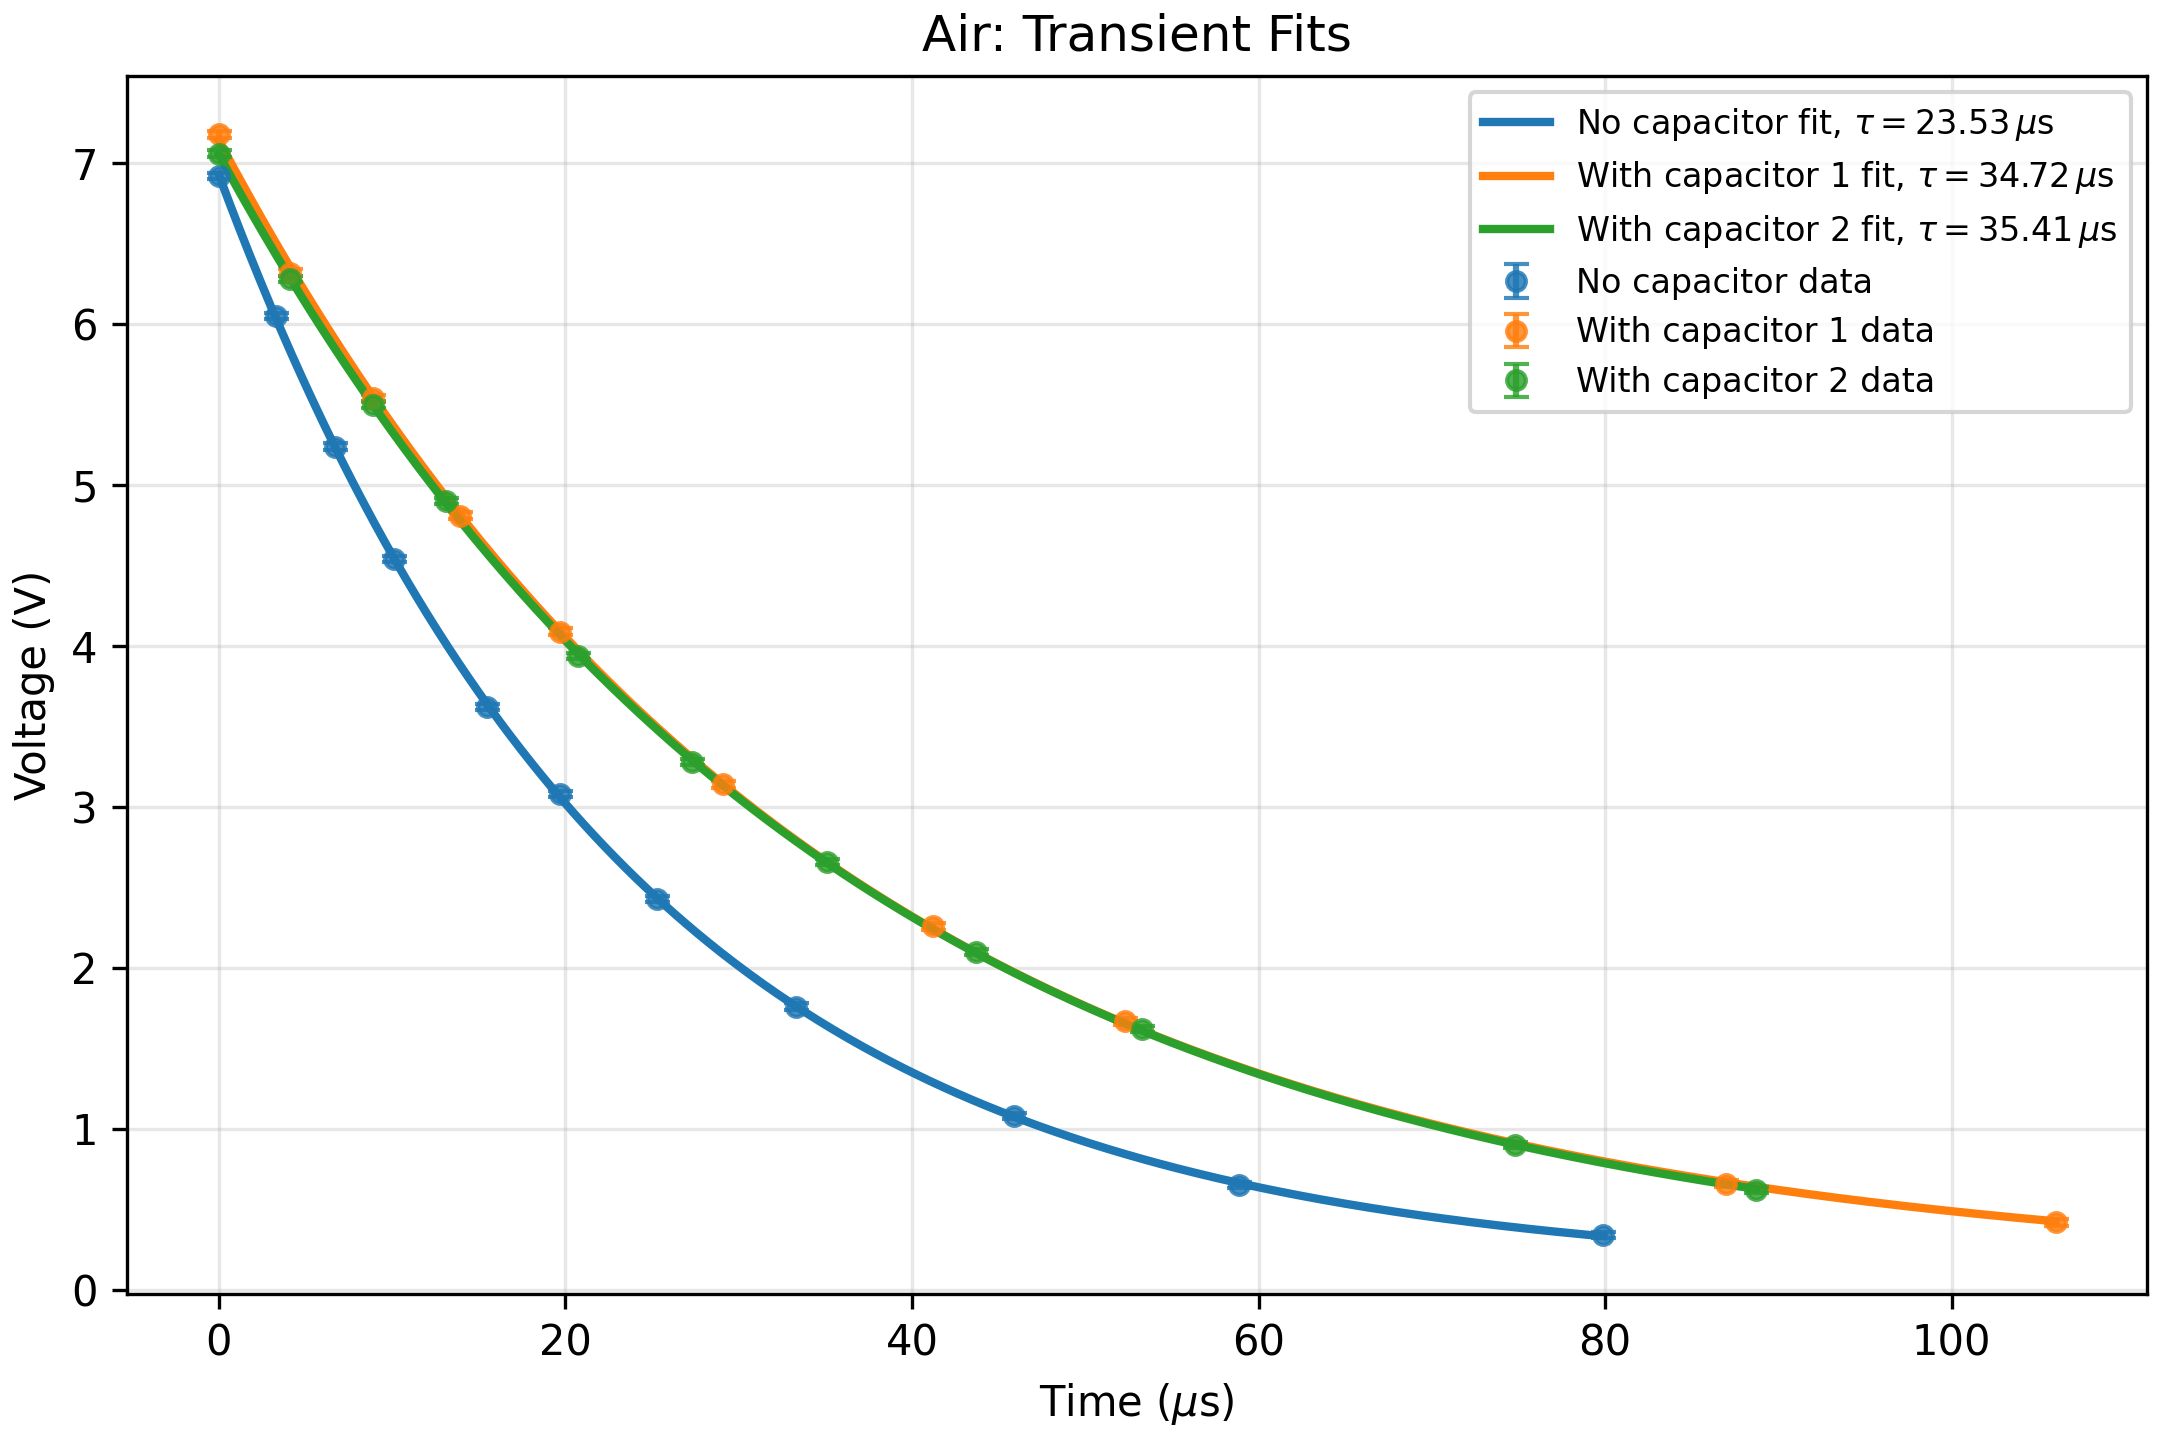
\includegraphics[width=0.88\textwidth]{air_transient_fit.png}
    \caption{Air transient fits. Error bars show the assigned vertical uncertainty for each run.}
\end{figure}

\begin{figure}[H]
    \centering
    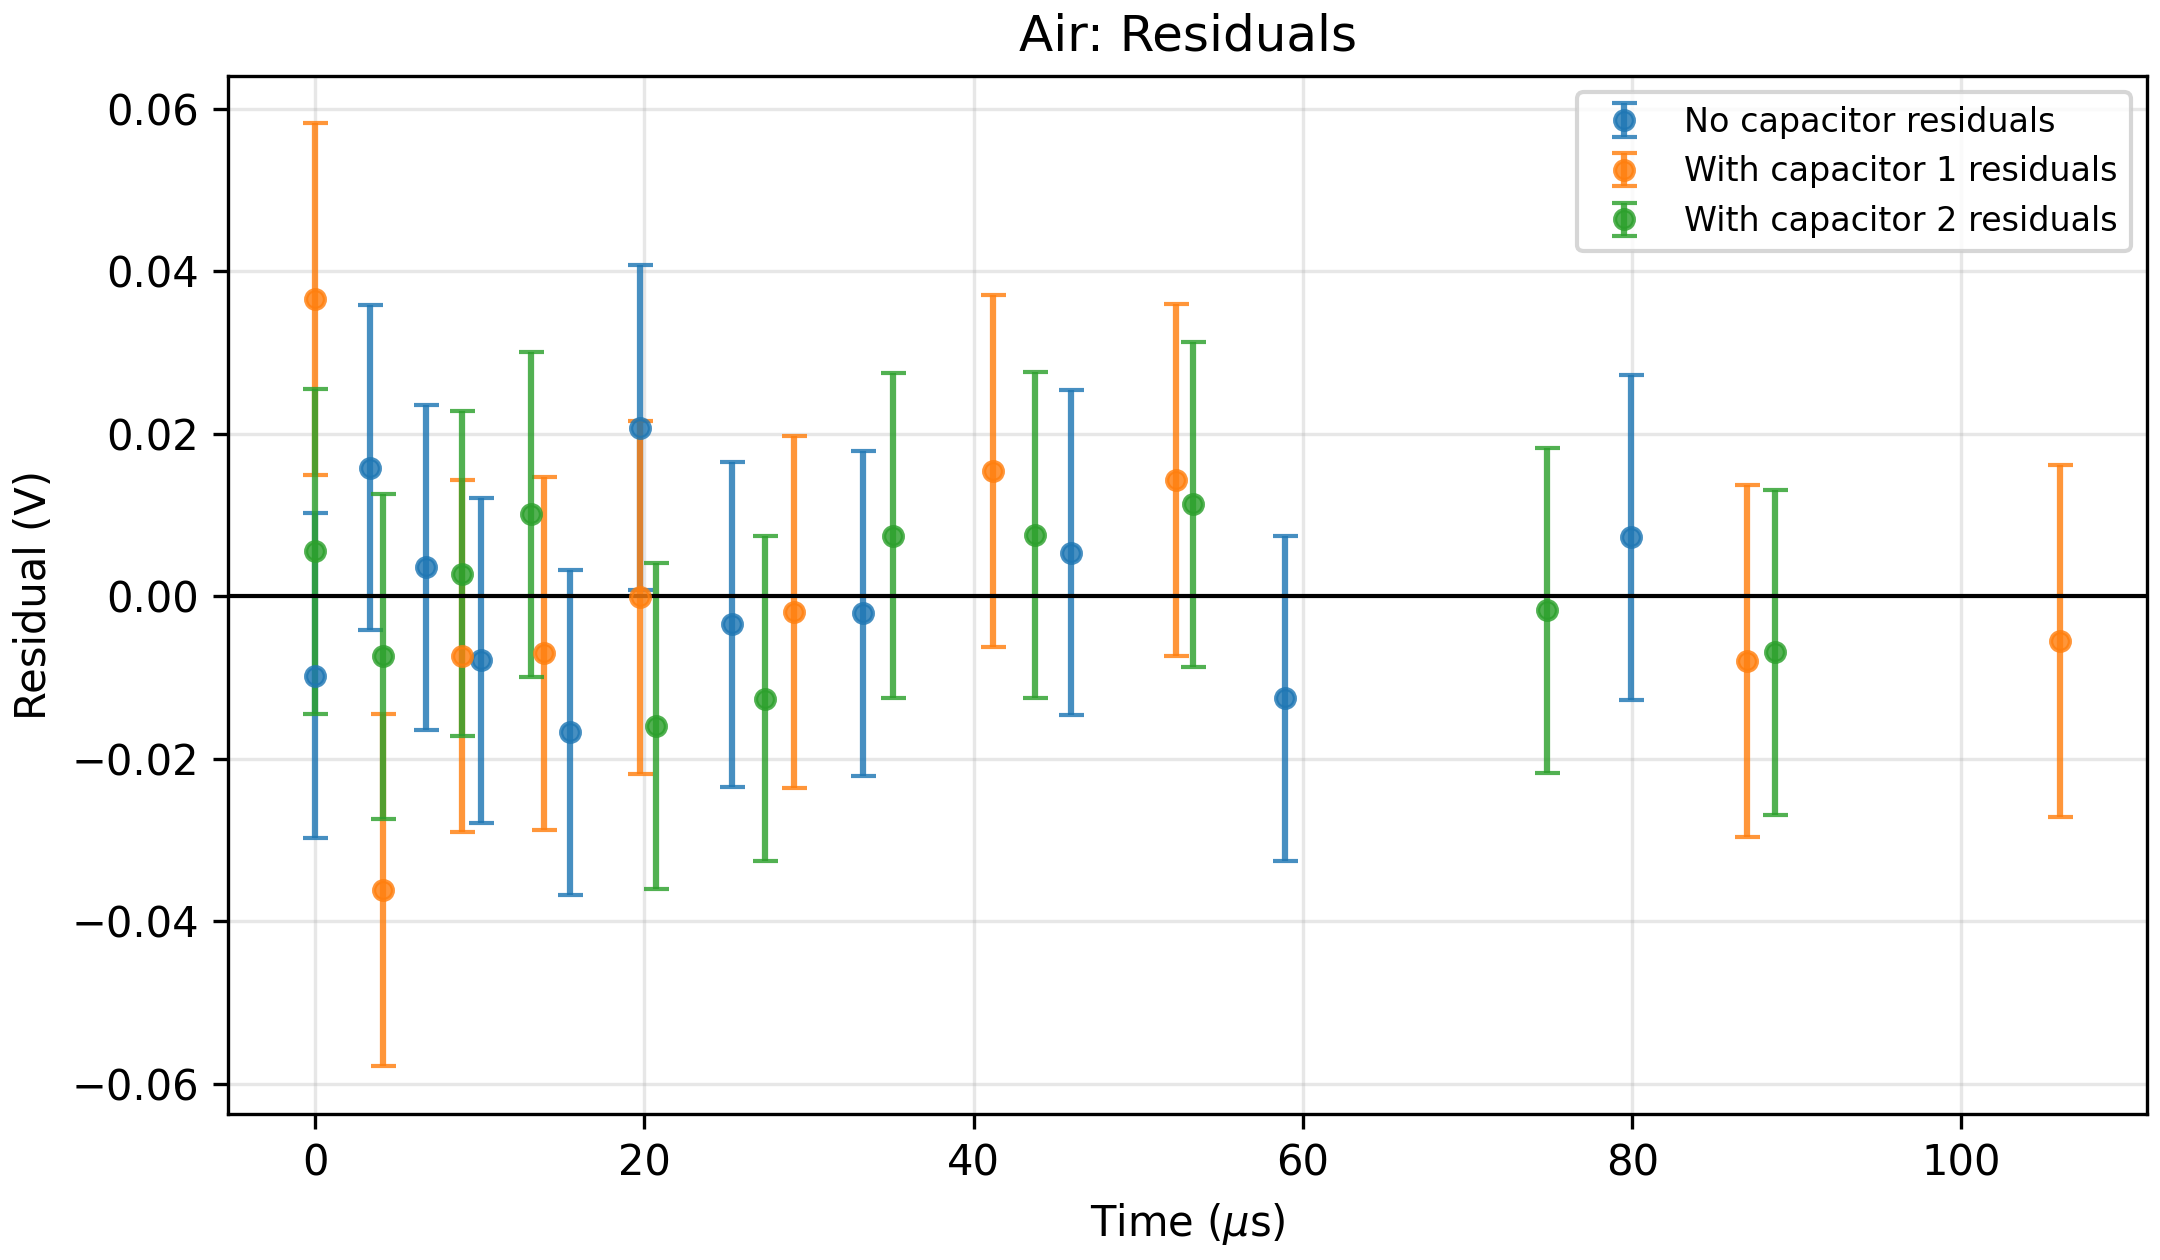
\includegraphics[width=0.88\textwidth]{air_transient_residuals.png}
    \caption{Air residuals for the exponential fits.}
\end{figure}

\begin{figure}[H]
    \centering
    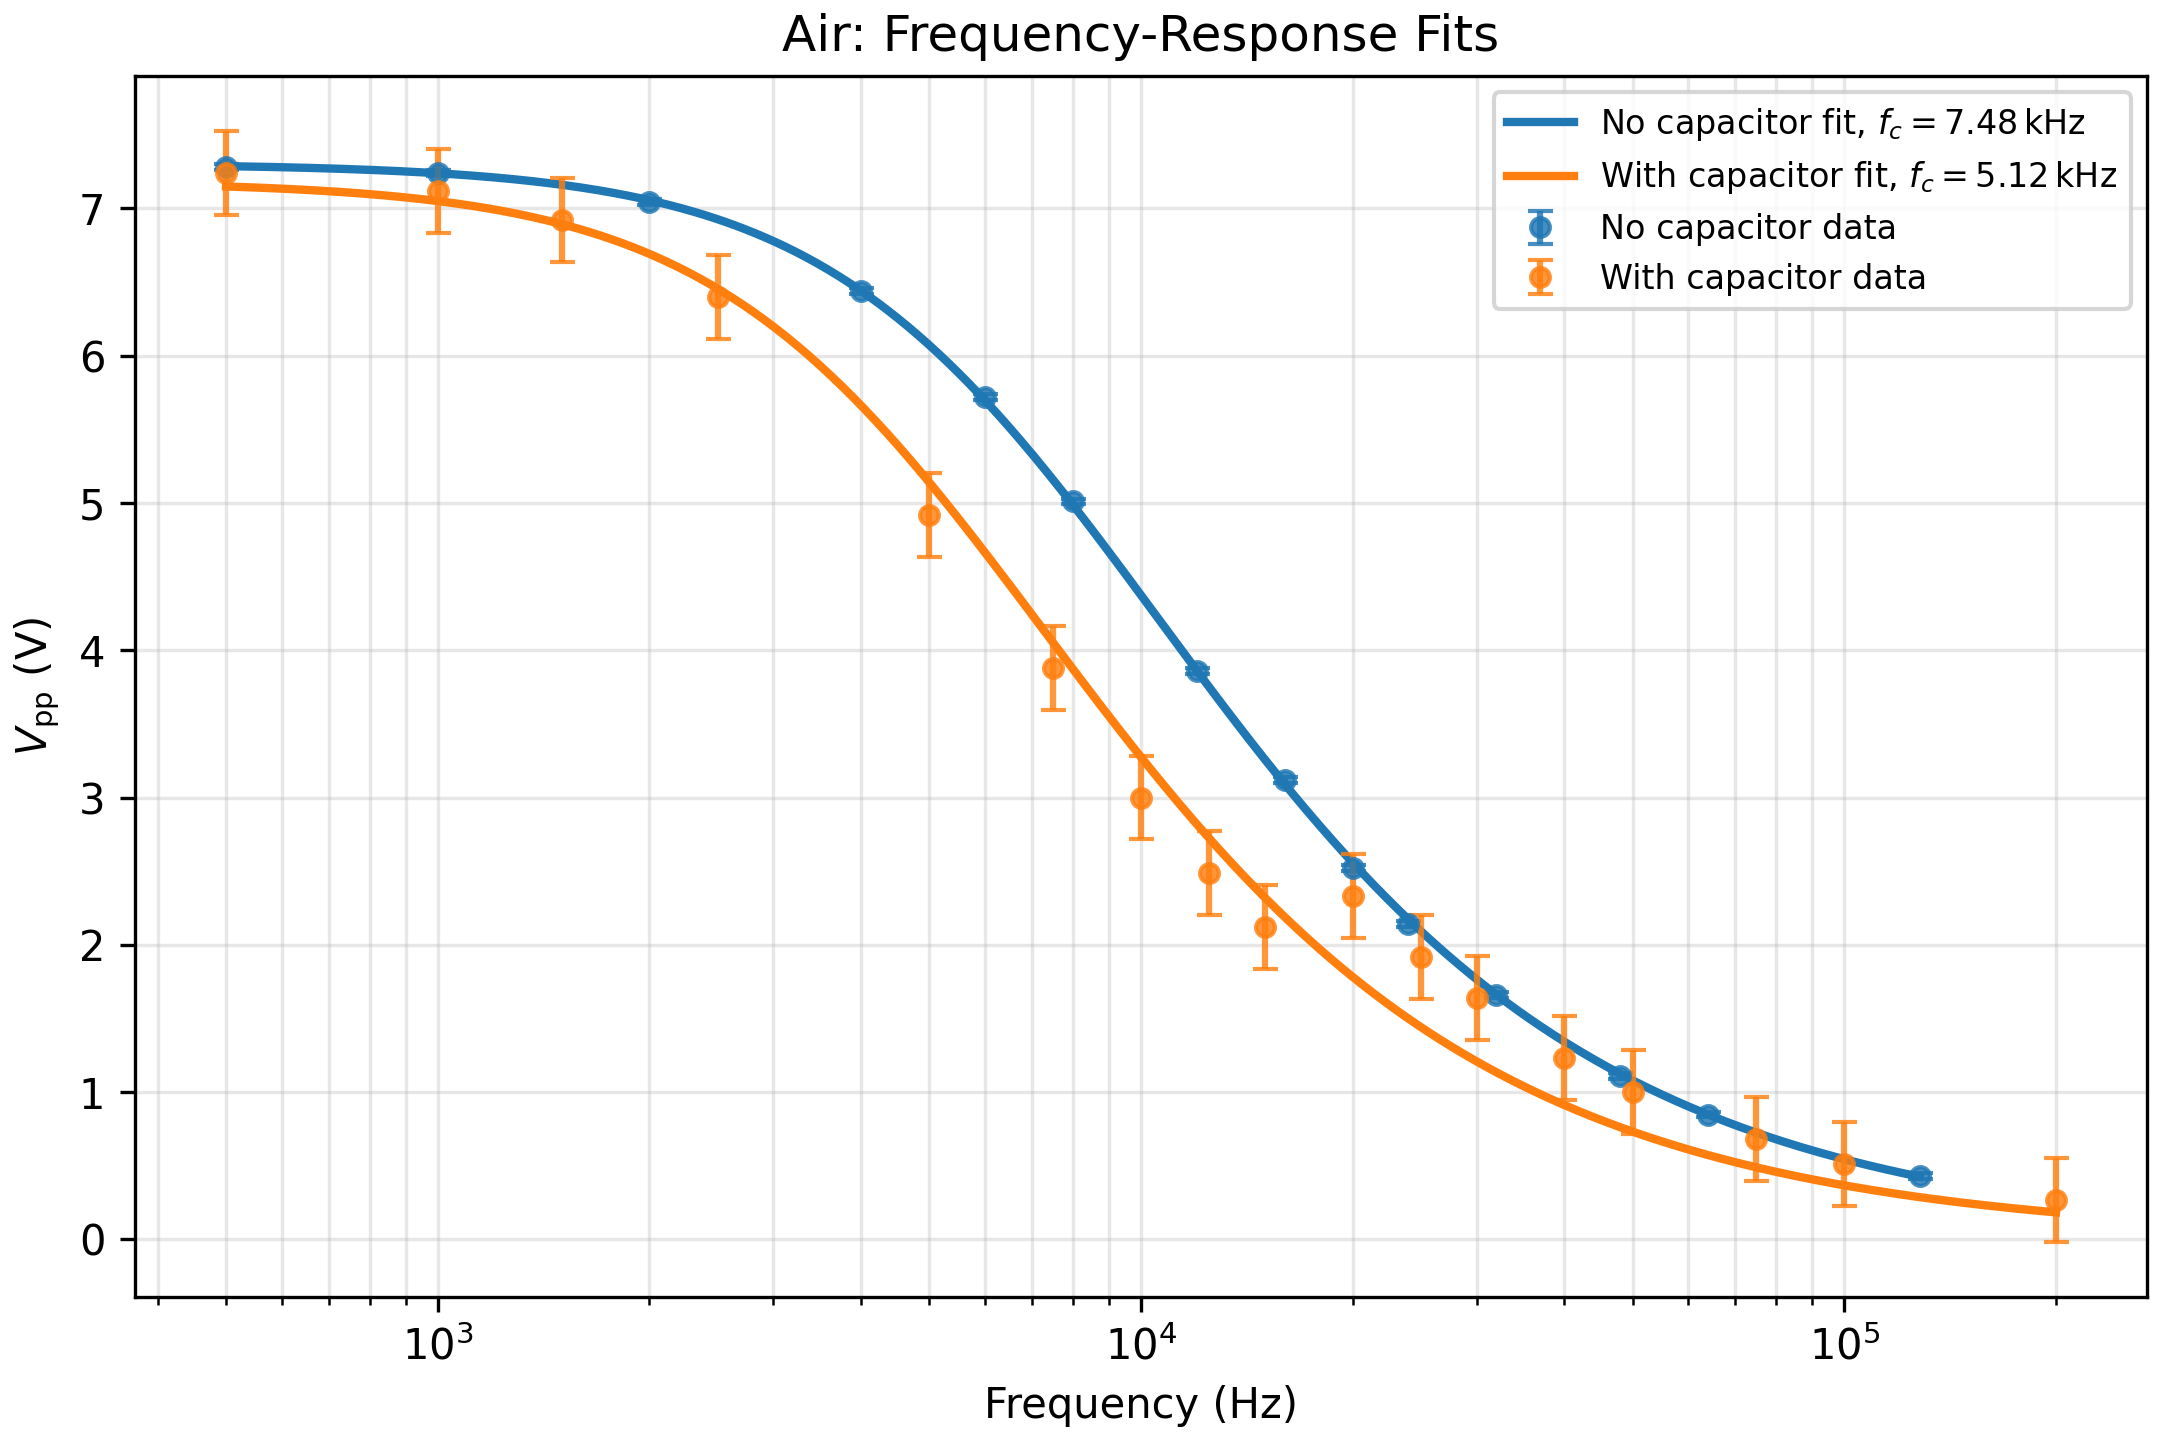
\includegraphics[width=0.88\textwidth]{air_frequency_response_fit.png}
    \caption{Air frequency-response fits using the low-pass model with the oscilloscope resistance included through $R_{\mathrm{eff}}$.}
\end{figure}

\begin{figure}[H]
    \centering
    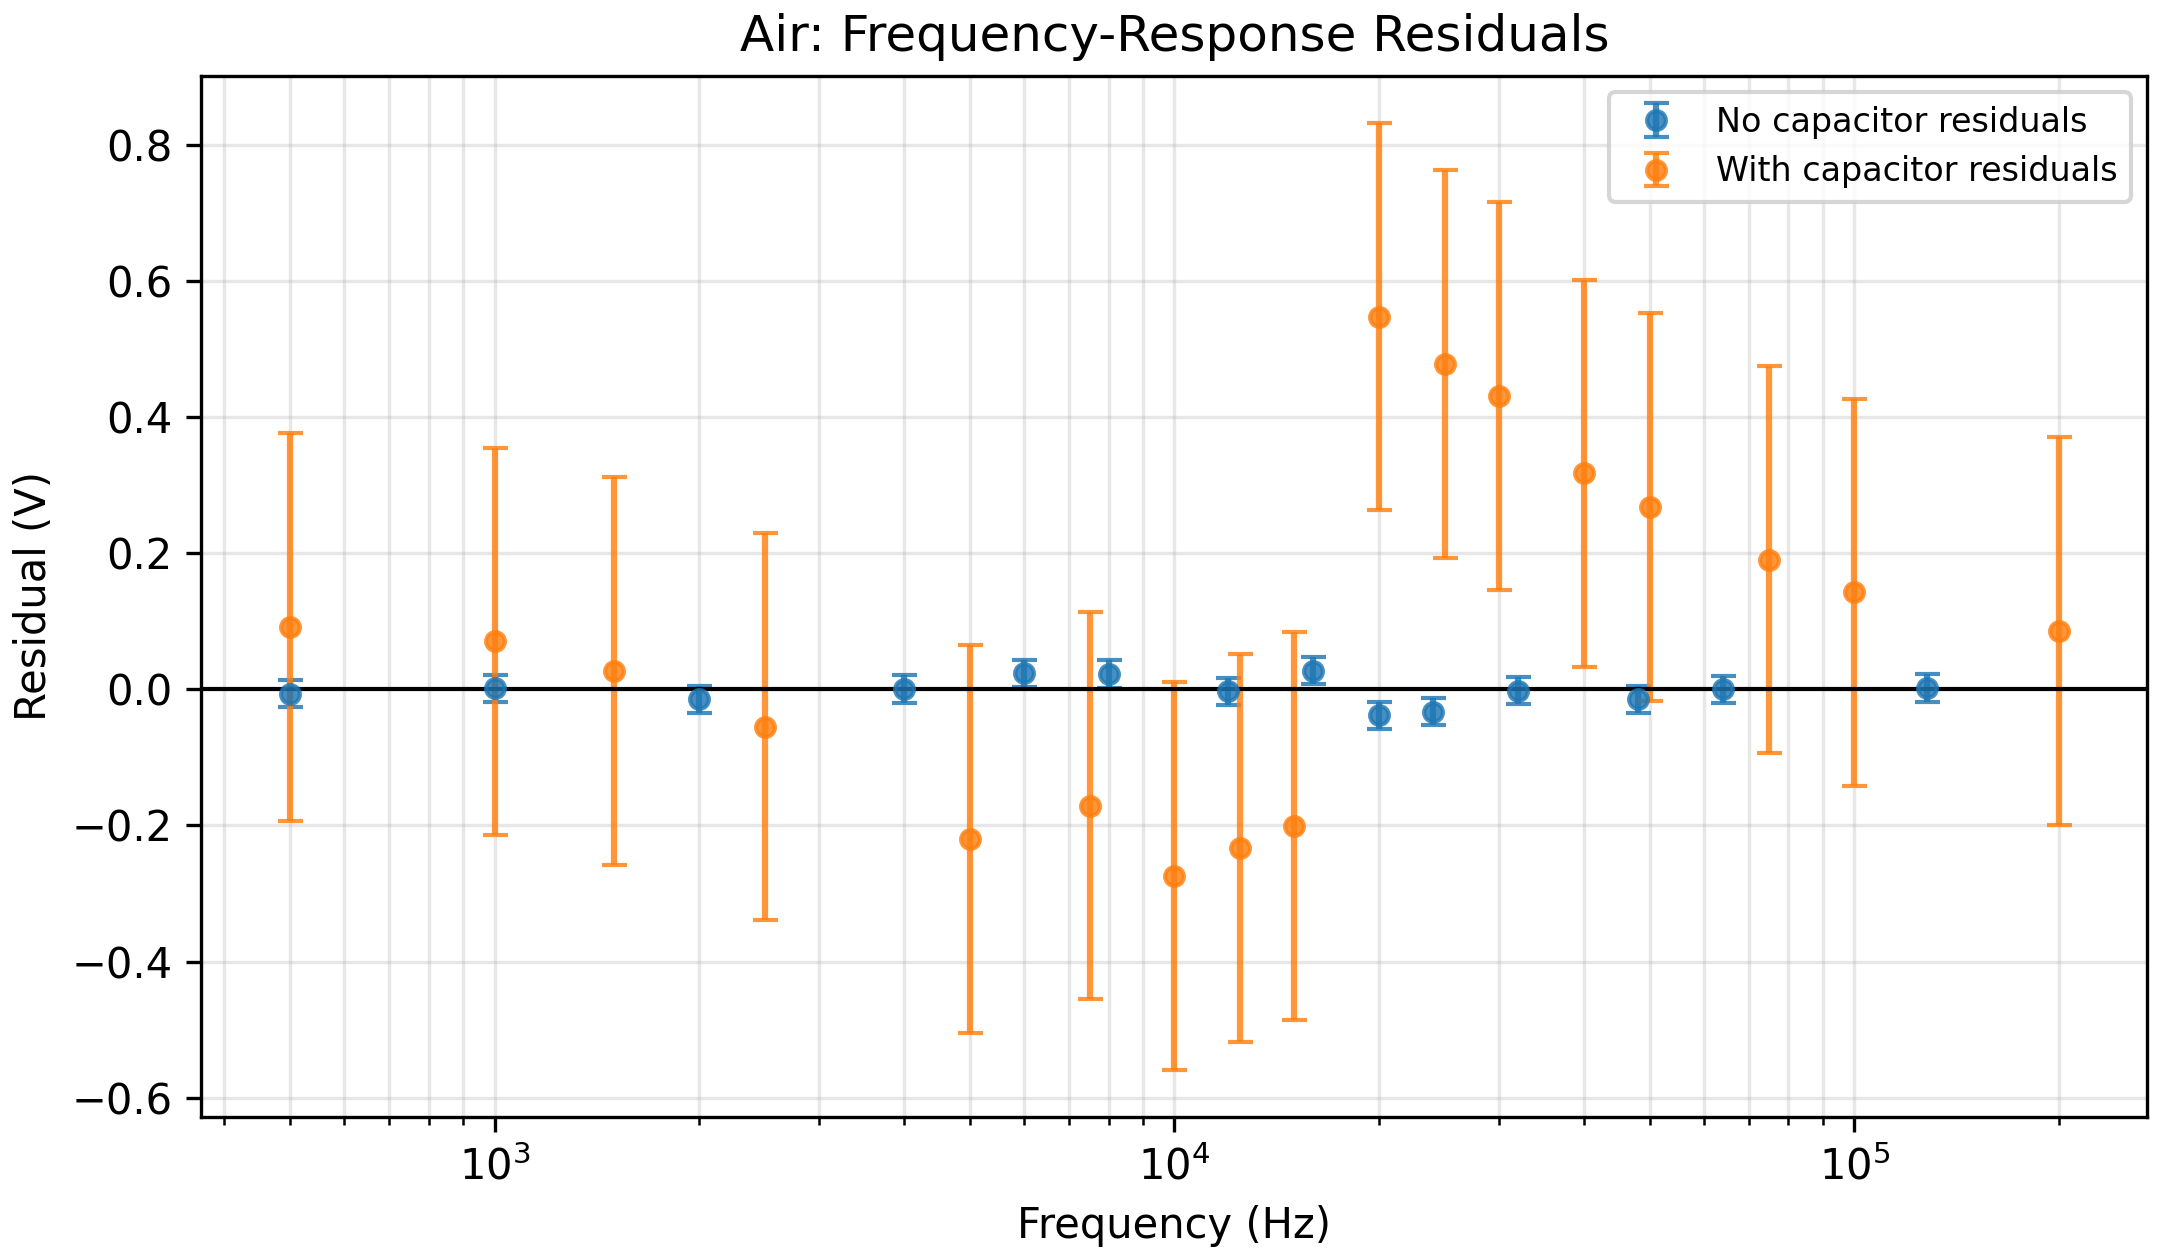
\includegraphics[width=0.88\textwidth]{air_frequency_response_residuals.png}
    \caption{Air frequency-response residuals. The with-capacitor sweep has visibly larger scatter than the no-capacitor sweep.}
\end{figure}

\begin{figure}[H]
    \centering
    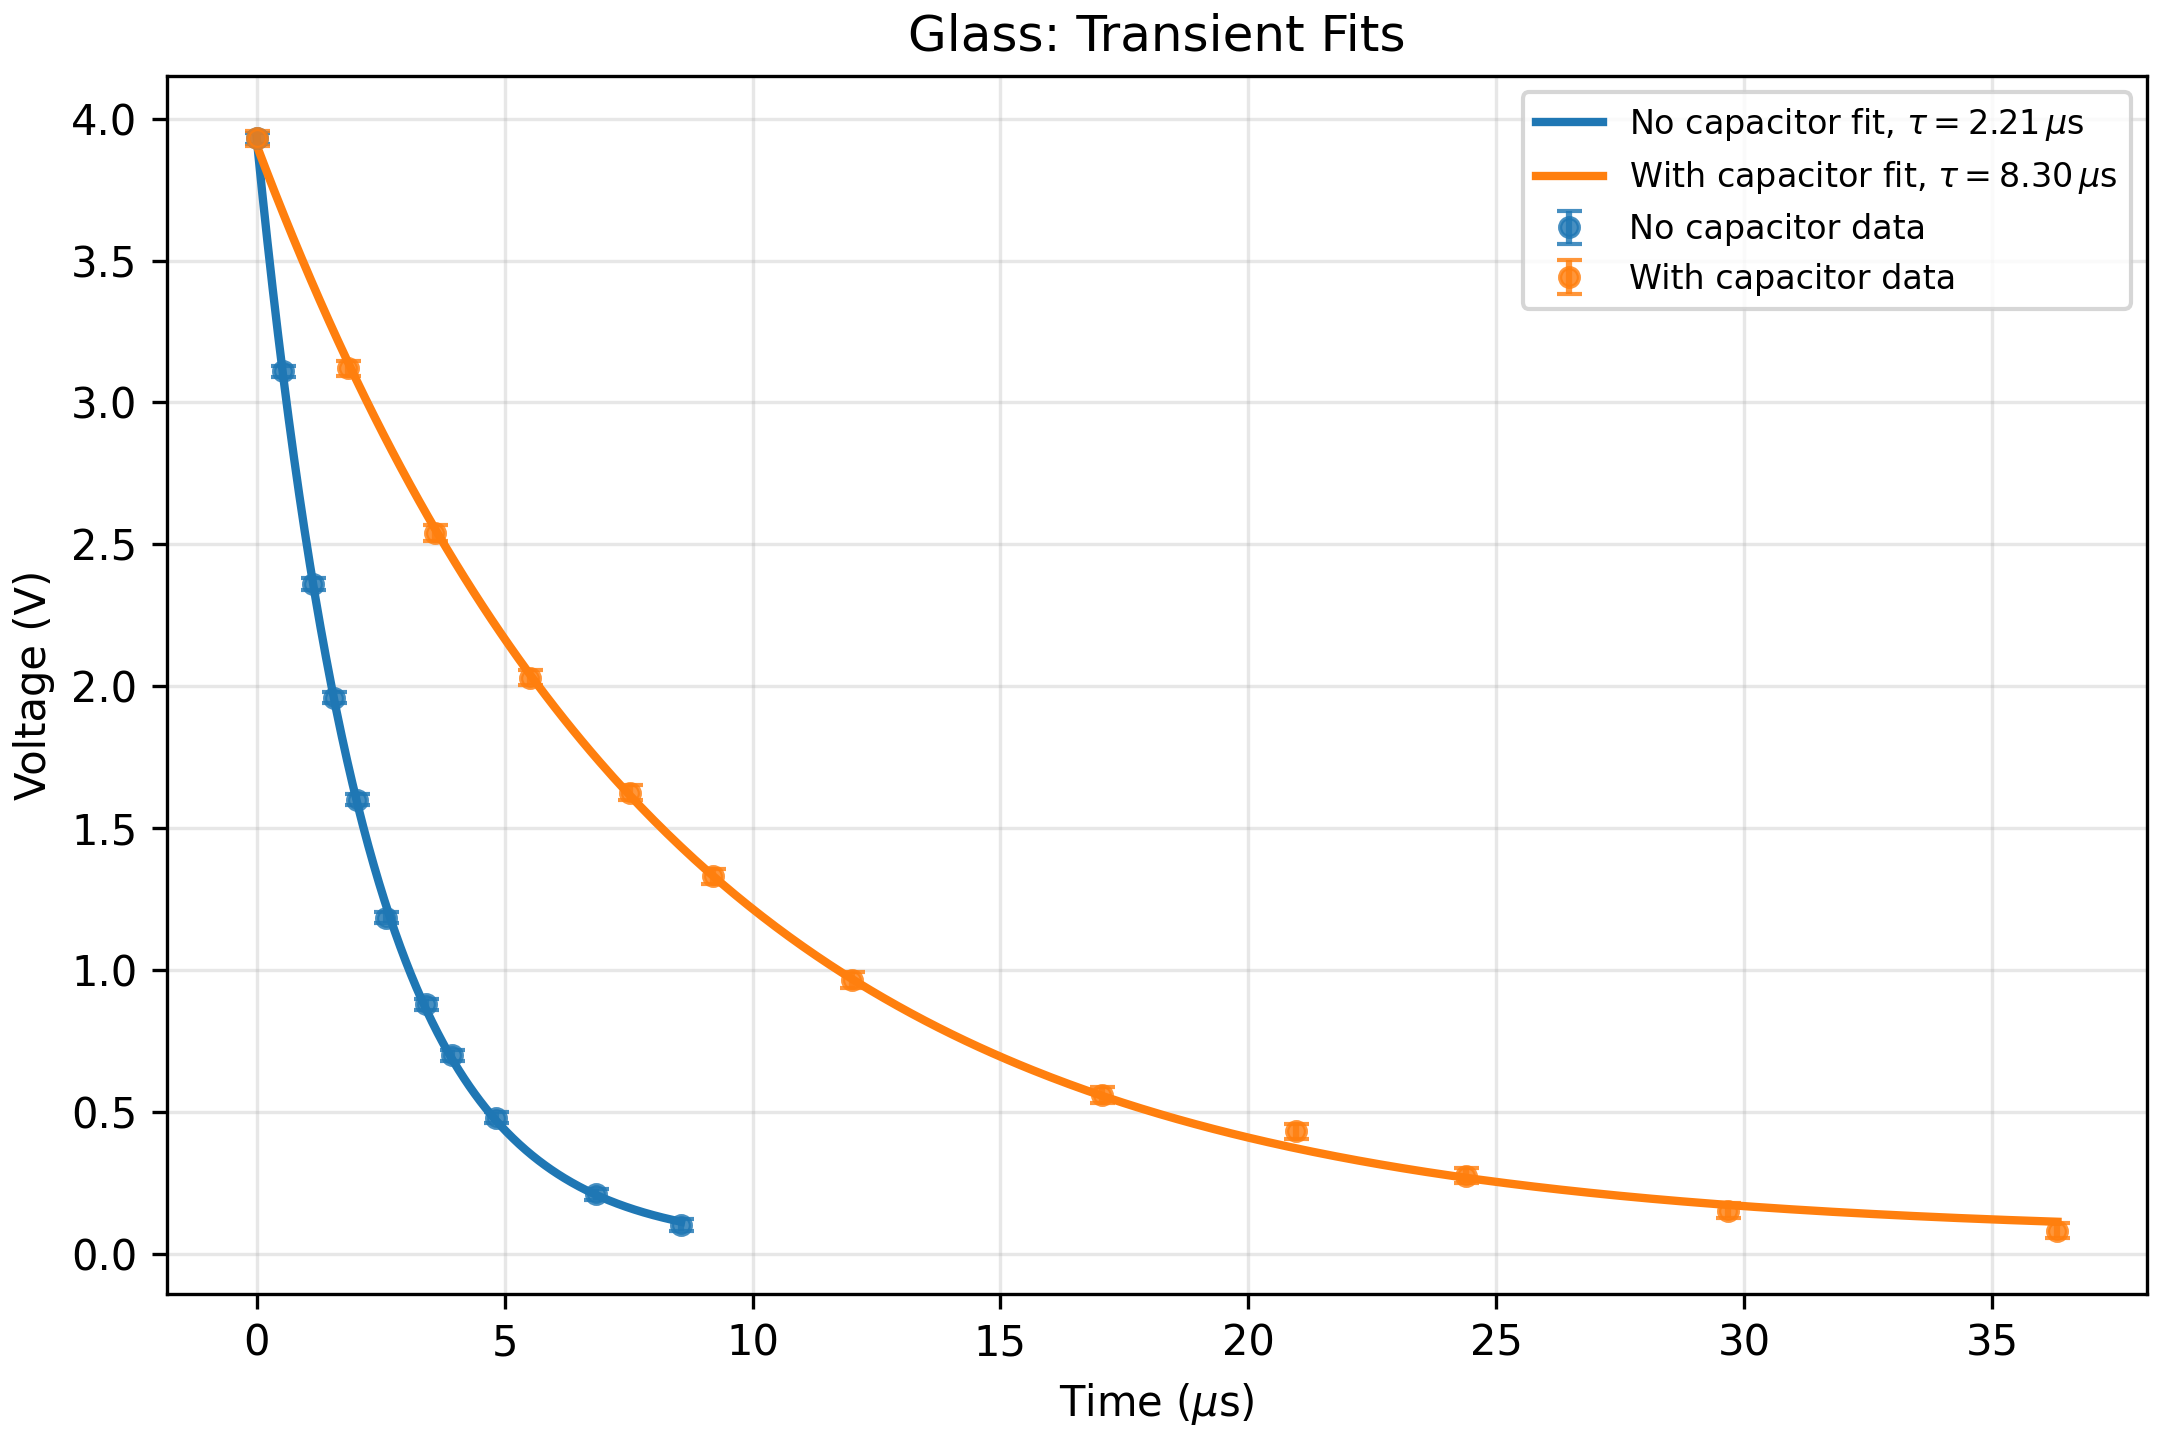
\includegraphics[width=0.88\textwidth]{glass_transient_fit.png}
    \caption{Glass transient fits. The longer ``With capacitor'' time constant indicates the additional capacitance from the glass-filled capacitor.}
\end{figure}

\begin{figure}[H]
    \centering
    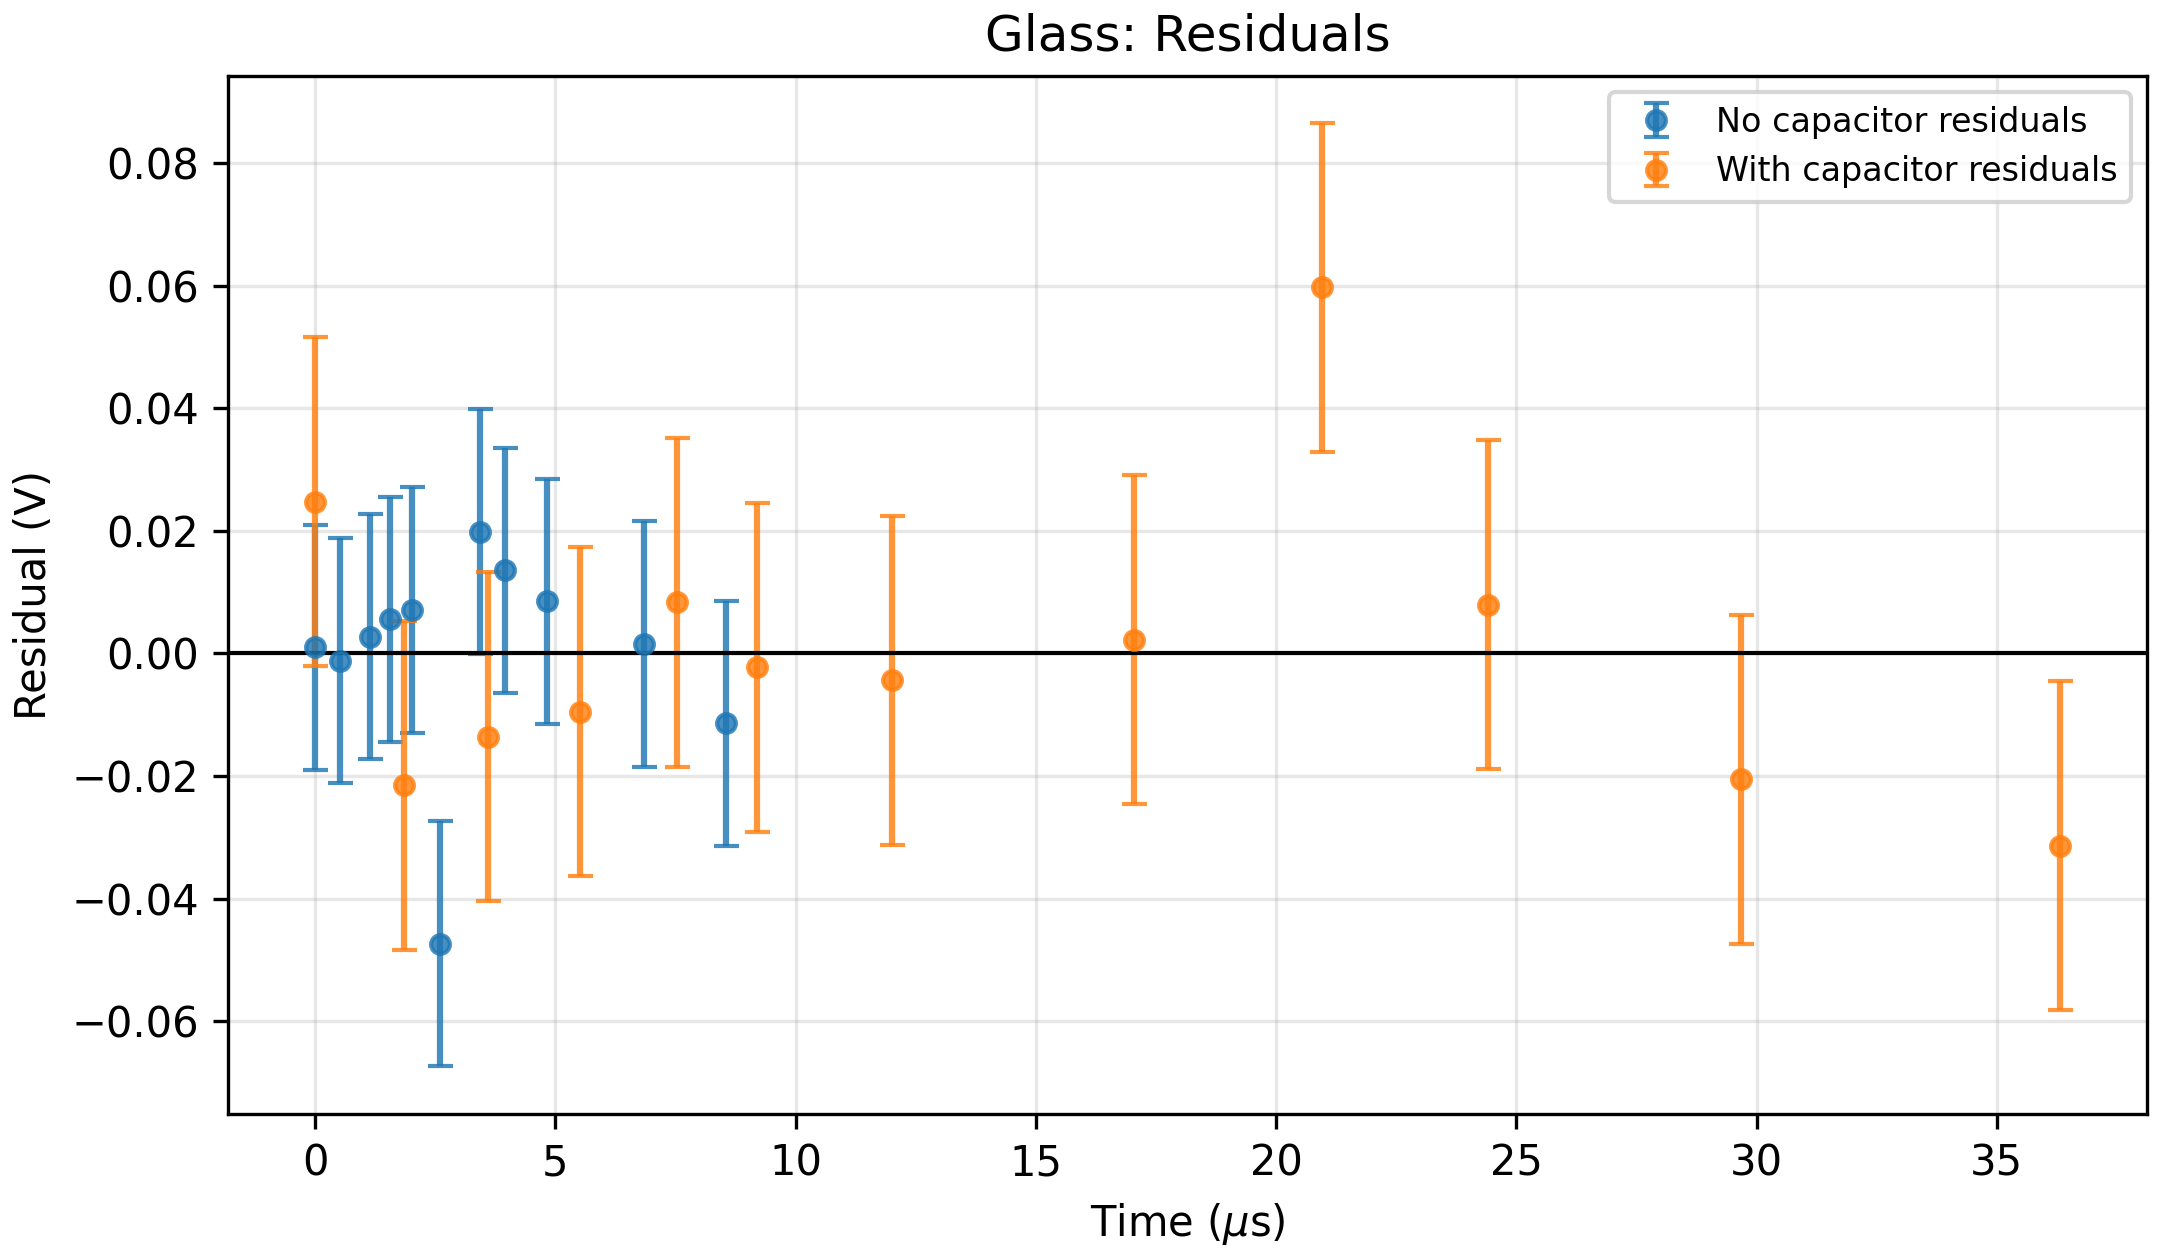
\includegraphics[width=0.88\textwidth]{glass_transient_residuals.png}
    \caption{Glass residuals for the exponential fits.}
\end{figure}

\begin{figure}[H]
    \centering
    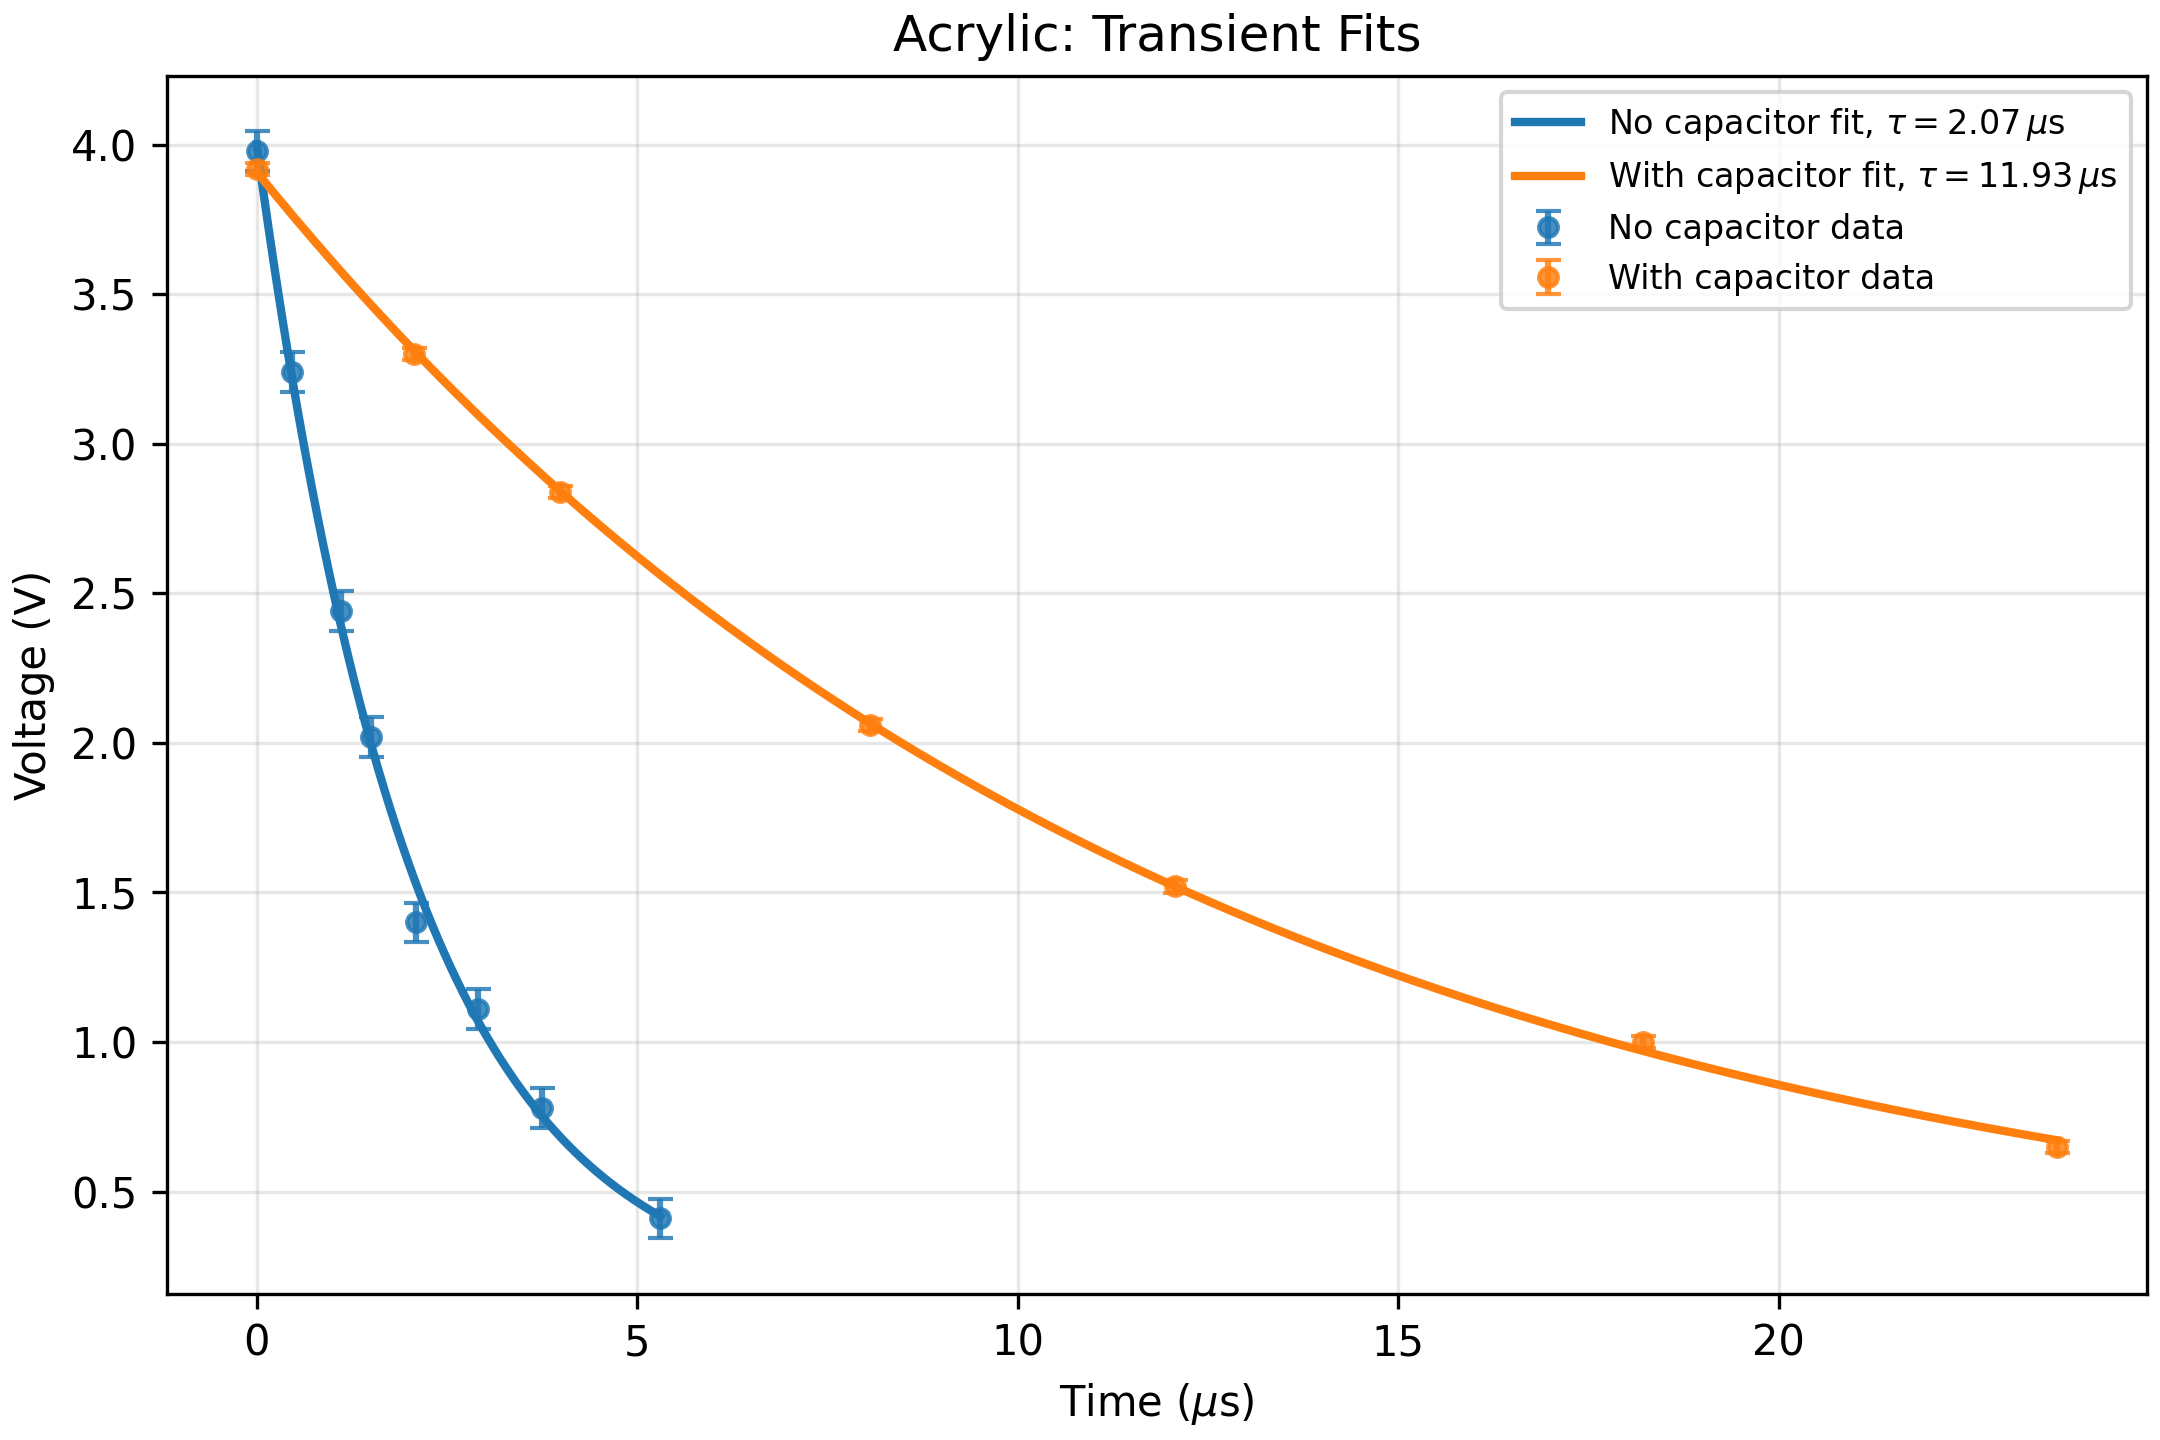
\includegraphics[width=0.88\textwidth]{acrylic_transient_fit.png}
    \caption{Acrylic transient fits.}
\end{figure}

\begin{figure}[H]
    \centering
    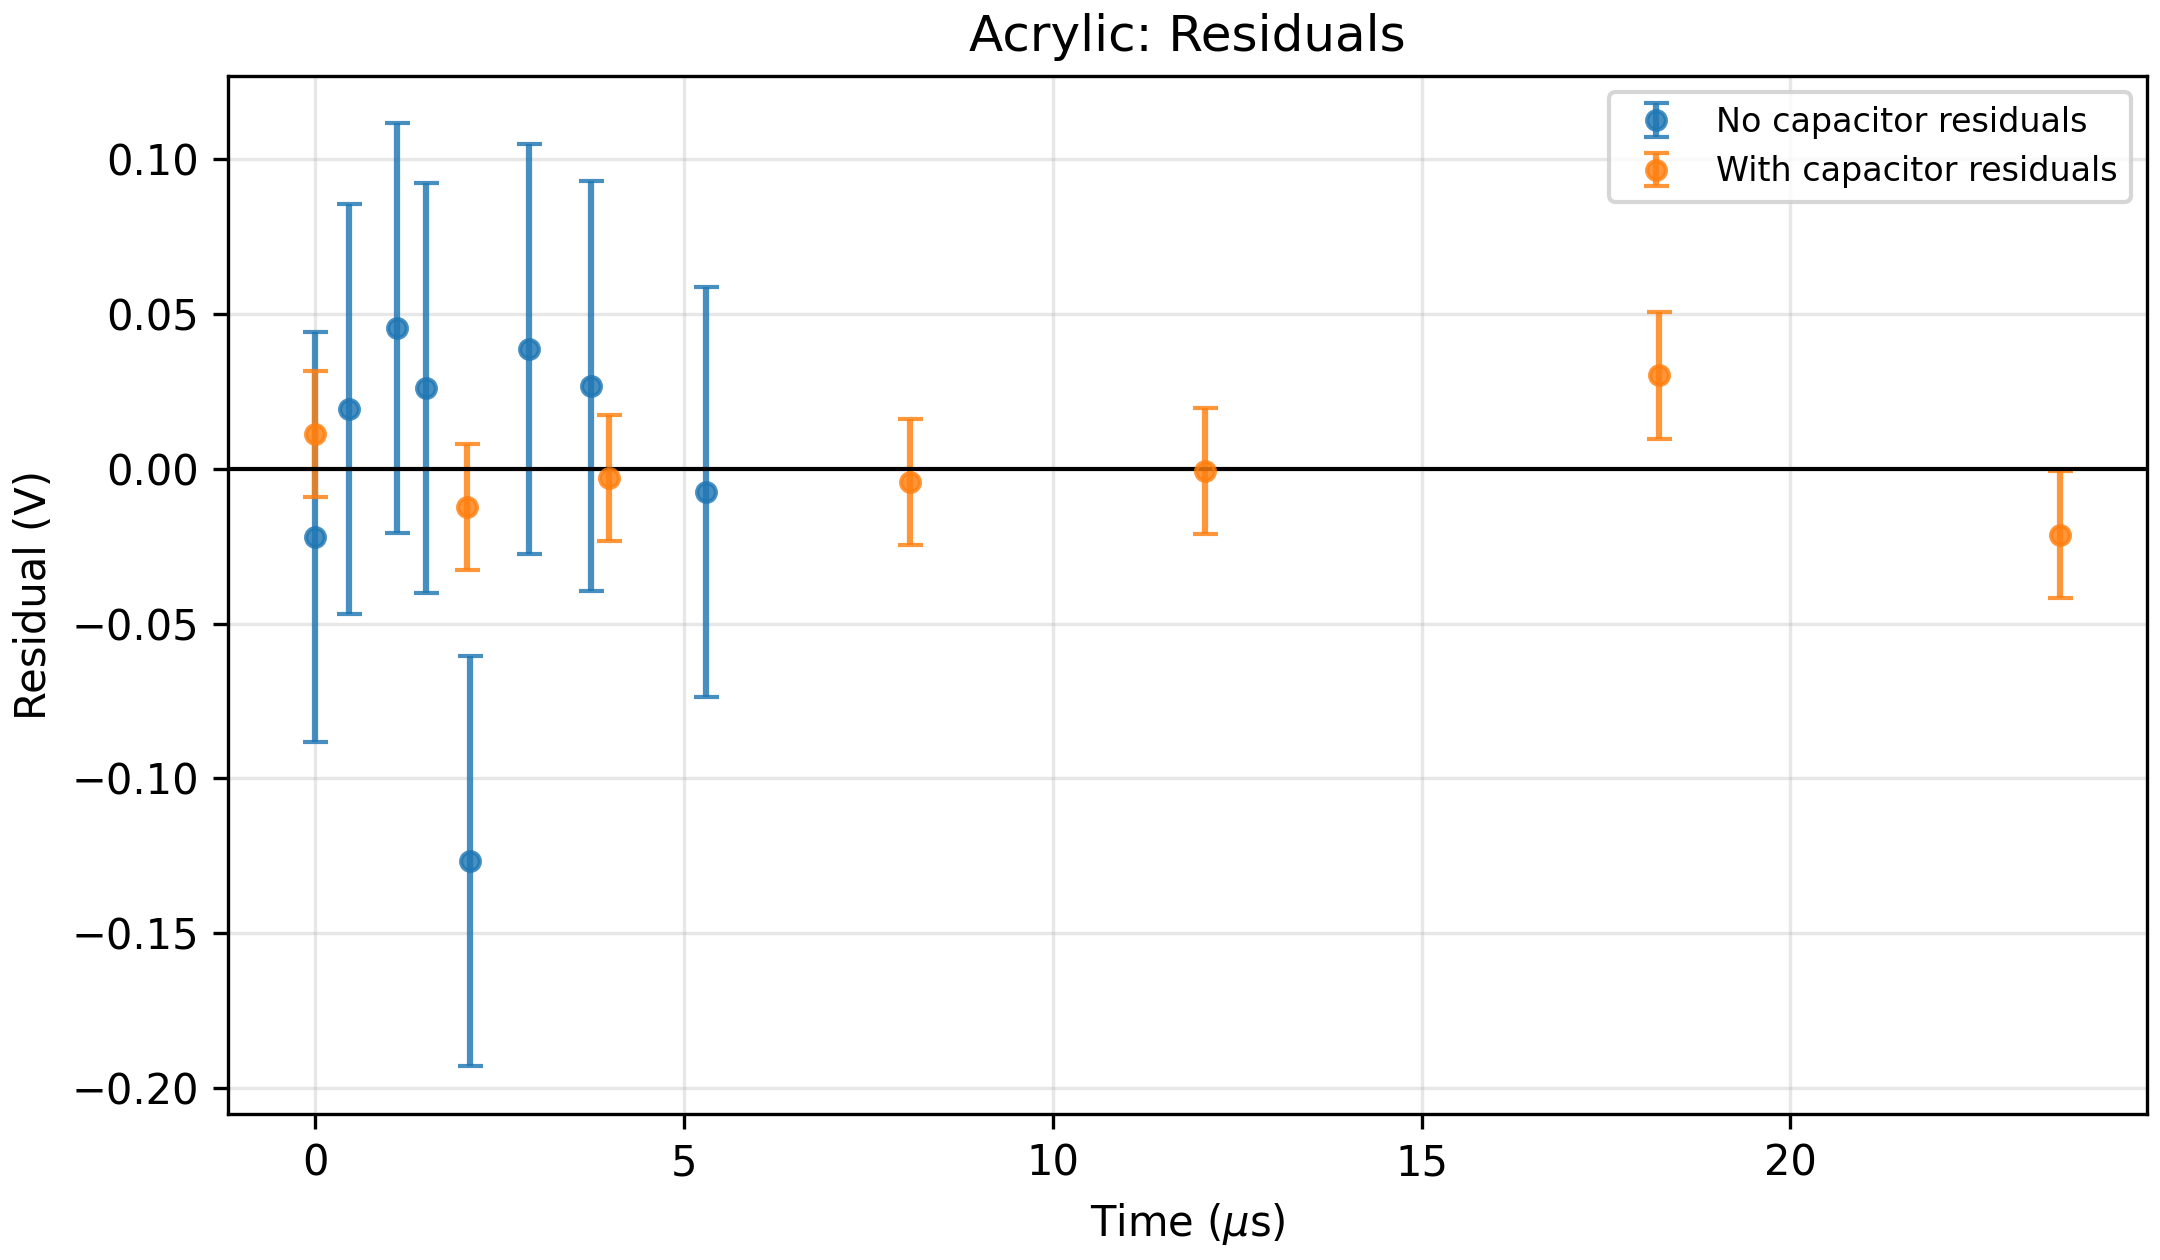
\includegraphics[width=0.88\textwidth]{acrylic_transient_residuals.png}
    \caption{Acrylic residuals for the exponential fits.}
\end{figure}

\section*{Analysis}

The key correction is that the oscilloscope contributes both a parallel resistance and a baseline capacitance. If the oscilloscope were treated as an ideal voltmeter, the extracted capacitance would be biased because the discharge resistance would be too large. Including the $1.00~\mathrm{M}\Omega$ input resistance gives the effective resistances listed in the Methods section.

For the air measurement,
\begin{equation}
    C_{\mathrm{scope,air}} = 258.88 \pm 2.18~\mathrm{pF}.
\end{equation}
The two total capacitances with the air capacitor connected were
\begin{align}
    C_{\mathrm{total,air},1} &= 381.87 \pm 3.65~\mathrm{pF},\\
    C_{\mathrm{total,air},2} &= 389.46 \pm 3.94~\mathrm{pF}.
\end{align}
Subtracting the baseline gives
\begin{align}
    C_{\mathrm{air},1} &= 122.99 \pm 4.26~\mathrm{pF},\\
    C_{\mathrm{air},2} &= 130.58 \pm 4.50~\mathrm{pF}.
\end{align}
A weighted average of the two corrected trials gives
\begin{equation}
    C_{\mathrm{air}} = 126.57 \pm 3.79~\mathrm{pF},
\end{equation}
where the final uncertainty has been inflated by the square root of the weighted reduced chi-squared, $\chi^2_\nu=1.505$, because the two trials scatter slightly more than their formal uncertainties predict.

For glass, the no-capacitor baseline was
\begin{equation}
    C_{\mathrm{scope,glass}} = 227.19 \pm 3.06~\mathrm{pF},
\end{equation}
and the total capacitance with the glass capacitor connected was
\begin{equation}
    C_{\mathrm{total,glass}} = 854.14 \pm 14.35~\mathrm{pF}.
\end{equation}
Thus the corrected glass capacitance was
\begin{equation}
    C_{\mathrm{glass}} = 626.95 \pm 14.68~\mathrm{pF}.
\end{equation}
The glass fit and residual plot show no large curvature left after the exponential fit, so the RC model appears to capture the observed transient behavior well.

For acrylic, the no-capacitor baseline was
\begin{equation}
    C_{\mathrm{scope,acrylic}} = 212.57 \pm 14.14~\mathrm{pF},
\end{equation}
and the total capacitance with the acrylic capacitor connected was
\begin{equation}
    C_{\mathrm{total,acrylic}} = 1228.09 \pm 35.91~\mathrm{pF}.
\end{equation}
This gives
\begin{equation}
    C_{\mathrm{acrylic}} = 1015.52 \pm 38.59~\mathrm{pF}.
\end{equation}
The acrylic no-capacitor run has the largest assigned voltage uncertainty, $\sigma_V=0.0663~\mathrm{V}$, because its initial residual scatter was larger than the $0.020~\mathrm{V}$ floor. This makes the acrylic baseline less precise than the air or glass baselines, but the corrected acrylic capacitance is still well separated from zero and much larger than the baseline correction.

The sine-wave frequency sweep gives an independent check on the air result. Fitting the no-capacitor sweep gives
\begin{equation}
    C_{\mathrm{scope,air,freq}} = 234.06 \pm 0.96~\mathrm{pF},
\end{equation}
and fitting the sweep with the circular capacitor connected gives
\begin{equation}
    C_{\mathrm{total,air,freq}} = 341.79 \pm 19.99~\mathrm{pF}.
\end{equation}
Subtracting the two gives
\begin{equation}
    C_{\mathrm{air,freq}} = 107.73 \pm 20.02~\mathrm{pF}.
\end{equation}
This agrees with the transient air value within one combined standard uncertainty. The frequency-response result is less precise because the with-capacitor sweep has larger point-to-point scatter, including a nonmonotonic point near $20~\mathrm{kHz}$, which is reflected in its assigned $\sigma_V=0.2848~\mathrm{V}$.

\begin{figure}[H]
    \centering
    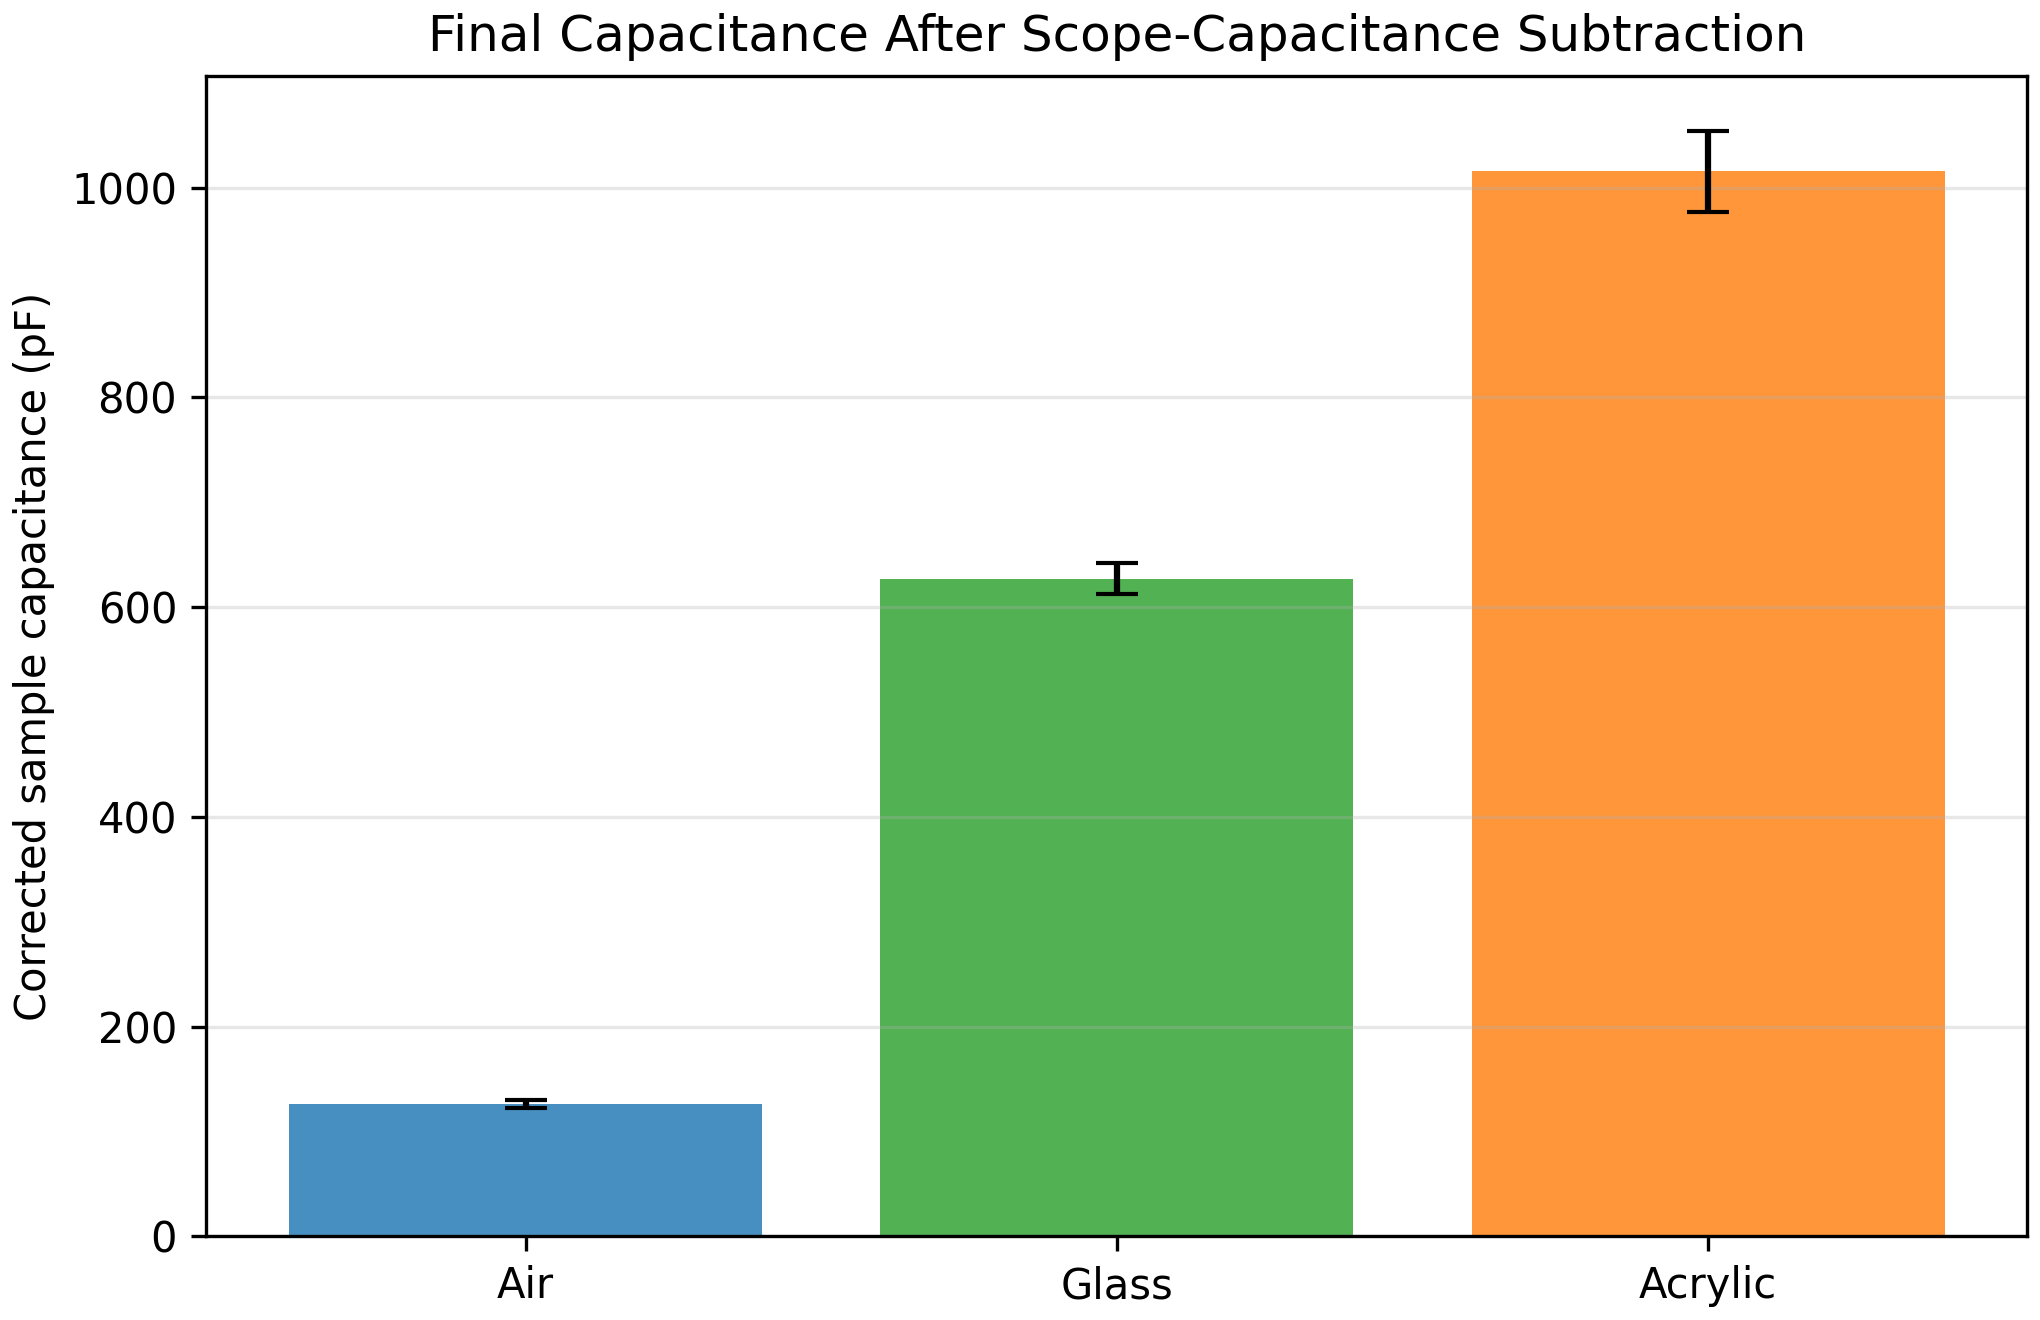
\includegraphics[width=0.82\textwidth]{final_capacitance_summary.png}
    \caption{Corrected capacitances after subtracting the corresponding no-capacitor oscilloscope baseline.}
\end{figure}

The residuals mostly fluctuate around zero rather than showing a large systematic curve, so the exponential transient model is appropriate for these measurements. The reduced chi-squared values should not be overinterpreted because the vertical uncertainties were estimated from the traces themselves, but they are useful consistency checks. The fits are strongest for the air and glass transient data. The acrylic no-capacitor baseline and the air with-capacitor frequency sweep are visibly noisier, but their larger uncertainties have been carried through the final values.

The geometry used to convert capacitance into permittivity is listed in Table 8. The air and glass geometry uncertainties were not independently estimated, so their tabulated permittivity uncertainties include only the capacitance uncertainty. For acrylic, the uncertainty in the overlap area was propagated from the two measured side lengths.

\begin{table}[H]
    \centering
    \caption{Geometry used for permittivity calculations.}
    \begin{tabular}{lcc}
        \toprule
        Material & Area $A$ ($\mathrm{m^2}$) & Thickness $d$ (m) \\
        \midrule
        Air & $\pi(0.100)^2=0.03142$ & 0.0025 \\
        Glass & $(0.34)(0.48)=0.1632$ & 0.00608 \\
        Acrylic & $(0.48\pm0.005)(0.33\pm0.01)=0.1584\pm0.0051$ & 0.0070 \\
        \bottomrule
    \end{tabular}
\end{table}

\begin{table}[H]
    \centering
    \caption{Permittivity values from the corrected transient capacitances.}
    \begin{tabular}{lccc}
        \toprule
        Material & $C$ (pF) & $\epsilon$ (F/m) & $\kappa$ \\
        \midrule
        Air & $126.57\pm3.79$ & $(1.007\pm0.030)\times10^{-11}$ & $1.14\pm0.03$ \\
        Glass & $626.95\pm14.68$ & $(2.336\pm0.055)\times10^{-11}$ & $2.64\pm0.06$ \\
        Acrylic & $1015.52\pm38.59$ & $(4.488\pm0.223)\times10^{-11}$ & $5.07\pm0.25$ \\
        \bottomrule
    \end{tabular}
\end{table}

Using the frequency-response air capacitance instead gives
\begin{equation}
    \epsilon_{\mathrm{air,freq}} = (8.57 \pm 1.59)\times10^{-12}~\mathrm{F/m},
    \qquad
    \kappa_{\mathrm{air,freq}} = 0.97 \pm 0.18,
\end{equation}
which is closer to the expected air value than the transient-only result, though with a much larger uncertainty.

\begin{figure}[H]
    \centering
    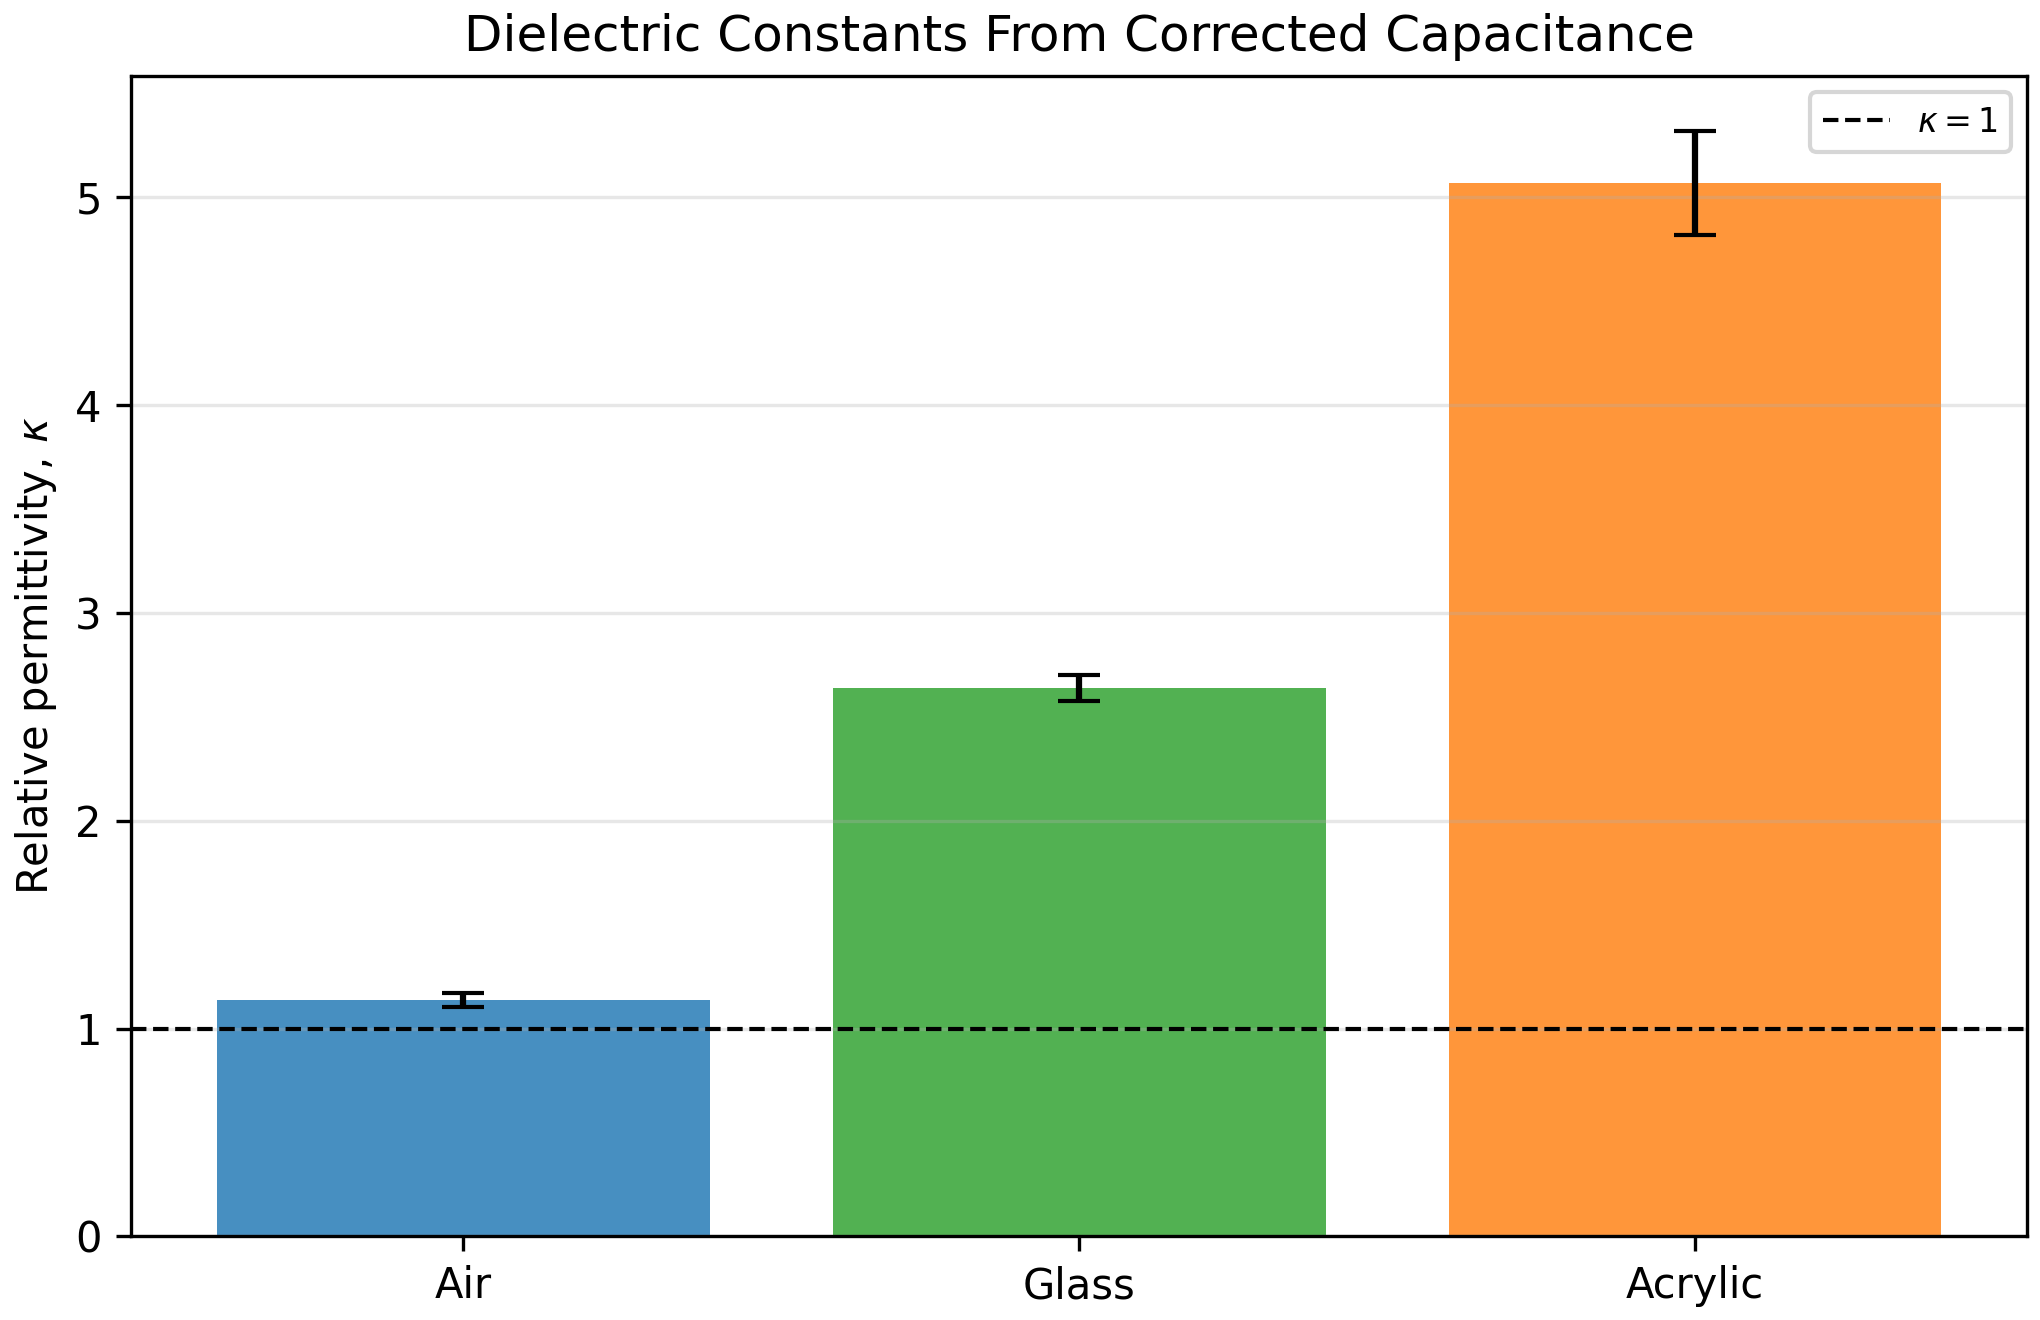
\includegraphics[width=0.82\textwidth]{permittivity_summary.png}
    \caption{Relative permittivities computed from the corrected transient capacitances and measured geometries.}
\end{figure}

\section*{Summary}

The oscilloscope correction changed the analysis in two ways: the discharge resistance was the parallel combination of the external resistor and the $1.00~\mathrm{M}\Omega$ oscilloscope resistance, and each no-capacitor run was treated as a baseline capacitance to subtract from the matching with-capacitor run. After these corrections, the measured capacitances were
\begin{align}
    C_{\mathrm{air}} &= 126.57 \pm 3.79~\mathrm{pF},\\
    C_{\mathrm{glass}} &= 626.95 \pm 14.68~\mathrm{pF},\\
    C_{\mathrm{acrylic}} &= 1015.52 \pm 38.59~\mathrm{pF}.
\end{align}
The frequency-response sweep gives an independent air value, $C_{\mathrm{air,freq}}=107.73\pm20.02~\mathrm{pF}$, consistent with the transient result. Using the measured geometries, the corresponding relative permittivities from the transient data are
\begin{align}
    \kappa_{\mathrm{air}} &= 1.14 \pm 0.03,\\
    \kappa_{\mathrm{glass}} &= 2.64 \pm 0.06,\\
    \kappa_{\mathrm{acrylic}} &= 5.07 \pm 0.25.
\end{align}
The residual plots support the RC models for the present data. The main remaining limitations are the hand-read oscilloscope values, the lack of independent point-by-point uncertainty estimates, scatter in the with-capacitor frequency sweep, and geometry uncertainties not fully captured for the air and glass capacitors.

\end{document}
